\documentclass[twocolumn]{class}


\addbibresource{References.bib}

% add path to images
\graphicspath{ {./images/} }

\title{Integrative Network Analysis: \\ Unveiling Symptom-Disease Interactions and Enhancing Predictive Models}
\shorttitle{Integrative Network Analysis}

\github{https://github.com/DavideLigari01/financial-project}

\author{Andreoli C. • Ligari D. • Alberti A. • Scardovi M. }

\affil[1]{Department of Computer Engineering, Data Science, University of Pavia, Italy \newline\centering Course of Financial Data Science}

\keywords{Graph theory • Features Engineering • Community detection • Null models • Random forest • MLP }
\abstract{  
    This study addresses the complex challenge of deciphering the relationships between symptoms and diseases in healthcare, 
    a crucial aspect for accurate diagnosis and predictive analytics. Employing network analysis, we blend theoretical and empirical
    approaches to understand these relationships. Our work primarily focuses on exploring complex network configurations,
    utilizing bipartite models and non-weighted edges to identify significant patterns in disease-symptom interactions.
    A key aspect of our research is the application of novel metrics, inspired by Hidalgo's works from 2007 and 2009, 
    to classify symptoms based on their predictive power and diseases based on their symptomatological complexity. These metrics, along with others 
    like betweenness centrality and community based ones, are instrumental in refining our predictive models and provide a avenue for 
    computational complexity reduction.\\
    Building upon this foundation, we delve into predictive modeling, aspiring to surpass existing benchmarks in the field. 
    Our approach centers on three proven machine learning models—Logistic Regression, Random Forest, and Multi-Layer Perceptron—each chosen
    for their demonstrated effectiveness in disease prediction using symptomatic data, as evidenced in the studies by Kohli, Singh, and Uddin (2019). 
    Through this study, we aim to advance the understanding and capabilities in disease prediction, providing valuable insights for the healthcare sector,
    and to evaluate a graph-based approach for the computational complexity reduction of predictive models.
}
\firstauthor{Scardovi Ligari Alberti Andreoli}
\publicationdate{\today}


\begin{document}

\maketitle
\pagestyle{FirstPage}

\tableofcontents
% \nocite{dizdar_dns_2021}

% ------------------- START OF SECTIONS -------------------


% ------------------- Introduction -------------------

% Introduction to the medical problem and how it is currently addressed (some bibliography)
\section{Introduction}

\firstword{I}{n} the dynamic field of healthcare, understanding the intricate relationships between symptoms and diseases is crucial
for precise diagnosis and predictive analytics. This study delves into these complex interactions using network analysis,
blending theoretical frameworks with empirical data. Our objectives are twofold: to unravel the complexities of these
relationships and to identify key features that enhance predictive modeling, and facilitating computational efficiency improvement.\\
Central to our analysis are complex network configurations, where we employ bipartite models and non-weighted edges to discover significant patterns.
We use a range of network metrics, comparing our results with null models to ensure statistical reliability. Our application of community detection
algorithms reveals hidden structures and relationships among diseases, enriching our understanding.\\
We leveraged metrics based on the work of \citeauthor{Hidalgo_2009}~\cite{Hidalgo_2009} and \citeauthor{Hidalgo_2007}~\cite{Hidalgo_2007},
which help classify symptoms and diseases according to their predictive strength. These metrics, along with traditional ones like betweenness centrality,
are key in characterizing our predictive models.\\
Building on this analytical groundwork, we venture into predictive modeling with the goal of exceeding current benchmarks.
In line with research by \citeauthor{Kohli}~\cite{Kohli}, \citeauthor{Singh}~\cite{Singh}, and \citeauthor{Uddin2019Dec}~\cite{Uddin2019Dec},
which highlights the efficacy of Logistic Regression, Random Forest, and Multi-Layer Perceptron algorithms in disease prediction from symptomatic data,
we focus on these models for our analysis. Furthermore we propose a graph-based approach for computational complexity reduction.\\
\pagestyle{OtherPage}

% ------------------- Dataset -------------------

% Description of the dataset and its features (some plots and one hot encoding)
\section{Dataset}

The dataset used for this project is obtained from Kaggle and is available at the
\href{https://www.kaggle.com/datasets/dhivyeshrk/diseases-and-symptoms-dataset?select=Final_Augmented_dataset_Diseases_and_Symptoms.csv}{following link}.
It comprises disease names along with the symptoms reported by the respective patients.

\noindent
\textbf{Overview:} The dataset encompasses 773 unique diseases and 377 symptoms, resulting in approximately 246,000 rows.
It was artificially generated while preserving Symptom Severity and Disease Occurrence Possibility.

\noindent
\textbf{Data Encoding:} To facilitate model training, the dataset utilizes one-hot encoding for each symptom, transforming
categorical symptom data into a binary format.

\noindent
\textbf{Class Imbalance:} The original dataset exhibited significant class imbalance, with some classes having only one
sample and others containing thousands. We addressed this problem using Oversampling and Undersampling techniques,
and the details are further elaborated in Section \ref{sec:methodology_ML}\ref{subsec:preliminary_data_preparation}.

\noindent
\textbf{Data Cleaning:} To allow consistent Oversampling, classes (diseases) with fewer than three symptoms were excluded
from the dataset, resulting in the removal of 25 classes. Additionally, diseases with no symptoms and symptoms with
no associated diseases were deleted as well.




% ------------------- Goals -------------------

% Description of the goals of the project:

% - ML model to predict the disease
% - Network analysis to find the most important symptoms to reduce complexity, and enhance the available features

\section{Goals}

The final objective of this project is to develop a robust \textbf{machine learning model} capable of predicting
diseases based on reported symptoms. In pursuit of this goal, \textit{two specific objectives} are outlined,
both centered around \textbf{leveraging the network} structure:\\

\begin{enumerate}
      %space the list
      \setlength\itemsep{1em}
      \item \textbf{New Feature Extraction:} Exploiting the network characteristics and metrics, aiming to
            extract novel features that can enhance the predictive capabilities of the model.

      \item \textbf{Complexity Reduction:} Leveraging network information, we aim to reduce
            the number of symptoms, retaining only the most relevant ones. This strategic reduction aims to decrease
            training time while preserving the accuracy of the model.
\end{enumerate}

\vspace{0.4cm}
\noindent
By integrating these two objectives, the project aspires to not only advance the predictive capabilities of the machine
learning model but also optimize its efficiency in handling the complexities inherent in disease prediction based on symptoms.


% - ML model to predict the disease
% - Network analysis to find the most important symptoms to reduce complexity, and enhance the available features


% ------------------- Methodology and Results Network -------------------

% Methodology used (very technical)
\section{Network Methodology}
In this section there is a technical description of the methodology used to create and analyze the network.

\subsection{Network Creation}
Prior to graph creation, a preliminary data analysis was conducted to identify isolated nodes.
The analysis revealed the presence of several symptoms, precisely 52 out of 377, not associated with any disease.
Consequently, these isolated symptoms were removed from the graph as they do not contribute informative content.
Diseases without associated symptoms were also removed for the same reason.\\
Additionally, an analysis of the node degree distribution was performed to assess whether the distribution follows
a power law (see Section \ref{sec:results_network}\ref{subsubsec:power_law_ccdf}).\\
Finally, a bipartite graph was created where nodes represent symptoms (lightcoral) and diseases (blue),
and edges denote the presence of symptoms in diseases.
For simplicity, the graph is unweighted.
Figure~\ref{fig:bipartite_graph} illustrates the resulting bipartite graph. As showed, diseases tend to be peripheral,
while symptoms tend to be central. This observation arises from the fact that symptoms are shared by multiple diseases,
whereas diseases exhibit distinct symptoms. Furthermore, symptoms are fewer in number than diseases,
making it more likely for a symptom to be shared among multiple diseases.\\
Figure~\ref{fig:unipartite_graphs} presents the unipartite graphs of symptoms and diseases.
\begin{figure*}[thbp]
    \centering
    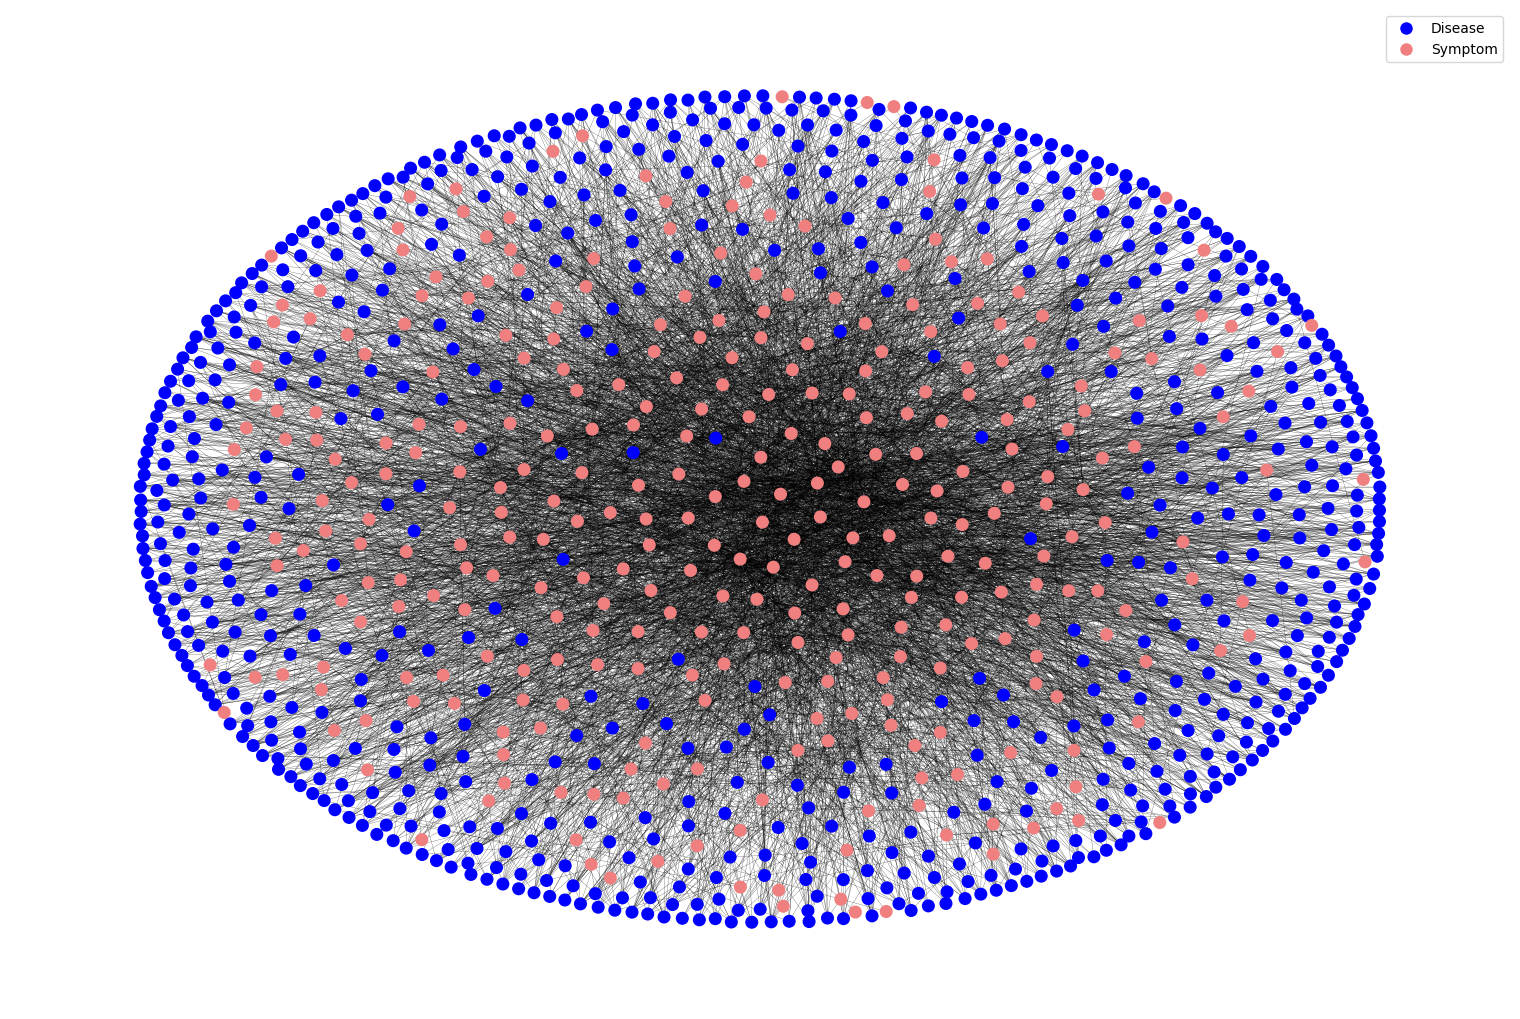
\includegraphics[width=.9\textwidth]{network.png}
    \caption{Visual representation of the symptom-disease bipartite graph.}\label{fig:bipartite_graph}
\end{figure*}
\noindent

\begin{figure}[H]
    \centering
    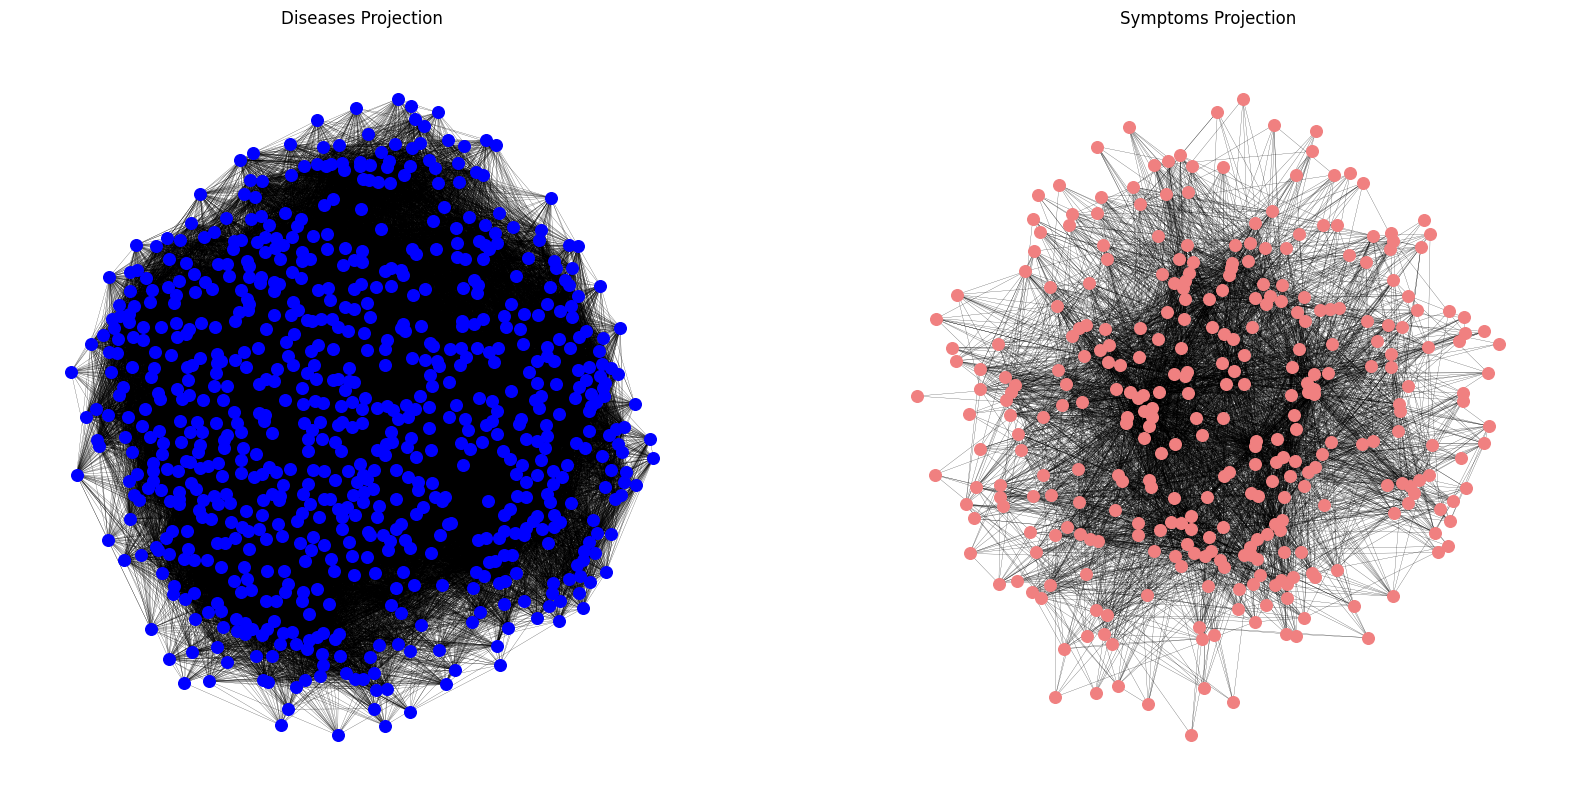
\includegraphics[width=.9\columnwidth]{unipartite_networks.png}
    \caption{Visual representation of symptom and disease unipartite graphs.}\label{fig:unipartite_graphs}
\end{figure}
\noindent

\subsection{Method of Reflections}

To identify influential nodes in the symptom-disease network, we introduce two indices that capture the relative importance of each actor.
The first index, referred to as the Symptom Influence (\textit{SI}) index, not only ranks symptom nodes based on their frequency (level-1)
but also considers whether a symptom is present in diseases affected by numerous other symptoms (level-2) or in diseases affected by only a few symptoms.\\
Conversely, the second index, known as the Disease Influence (\textit{DI}) index,
assesses the distinct symptoms related to a disease (level-1) and whether a disease exhibits symptoms that affect many other diseases (level-2).\\
In other words, level-1 of these indices quantifies the number of symptoms associated with a disease,
while level-2 measures the interconnectedness and broader impact of symptoms or diseases within the network.
For the Symptom Influence (\textit{SI}) index, level-2 takes into account the presence of a symptom across diseases,
shedding light on whether a particular symptom tends to co-occur with a wide range of other symptoms or is more specific to a subset of diseases.
This dual-level analysis provides a nuanced understanding of the significance of symptoms based not only on their individual prevalence (level-1)
but also on their associations with other symptoms across different diseases (level-2). Similarly, for the Disease Influence (\textit{DI}) index,
level-2 assesses the extent to which a disease's symptoms have ripple effects on other diseases, indicating the potential for cascading impacts within the network.\\
We adapt the level-\textit{N} indices following the approach of \citeauthor{Hidalgo_2007},\cite{Hidalgo_2007} and  \citeauthor{Hidalgo_2009},\cite{Hidalgo_2009}.
The level-\textit{N} indices are defined as:
\begin{equation}
    SI_{v, N} = \frac{1}{SI_{v, 1}} \sum_u W(v, u) DI_{u, N-1}
\end{equation}
\begin{equation}
    DI_{u, N} = \frac{1}{DI_{u, 1}} \sum_v W(v, u) SI_{v, N-1}
\end{equation}
\noindent
Here, $SI_{v, 1}$ and $DI_{u, 1}$ represent the level-1 indices, and $W(v,u)$ denotes the edge weight between symptom $v$ and disease $u$.
The level-1 indices are defined as follows:
\begin{equation}
    SI_{v, 1} = \sum_u W(v, u)
\end{equation}
\begin{equation}
    DI_{u, 1} = \sum_v W(v, u)
\end{equation}
\noindent
Since our network is not weighted ($W(v,u)=1$ if symptom $v$ is associated with disease $u$ and $W(v,u)=0$ otherwise),
$SI_{v,1}$ and $DI_{u,1}$ are equal to the degree of symptom $v$ and disease $u$, respectively.
\subsubsection*{Statistical Validation of SI and DI}

In our effort to identify significant nodes within the symptom-disease network,
we focus on discerning topological properties that hold statistical significance.
Our goal is to differentiate higher-order properties that are directly associated with local node features from those
that emerge from the intricate interactions among nodes.\\
Relevant studies~\citeauthor{Squartini_2011_a}~\cite{Squartini_2011_a, Squartini_2011_b} and~\citeauthor{Spelta_2023}~\cite{Spelta_2023}
highlight how higher-order network properties naturally capture structured group interactions.
Here, a `group' is defined as all players connected by a `hyperlink', representing the higher-order analog of a link.\\
The sampling of random graphs with specified properties plays a pivotal role in network analysis,
serving as fundamental null models for identifying patterns, including communities and motifs.\\
To statistically assess the significance of SI and DI, we adopt a hypothesis testing approach based on a null model.
Specifically, we posit \textbf{H0} as the hypothesis that SI and DI level-2 do not offer additional information compared to level-1,
and \textbf{H1} as the opposite.
To test these hypotheses, we generate 5000 random networks using a null model with the same level-1 properties as the original network.\\
With this ample set of null models, we assume that the distribution of SI and DI is Gaussian, leveraging the Central Limit Theorem (CLT).
For each null model, we calculate the mean ($\mu$) and standard deviation ($\sigma$) of SI and DI and compute the z-score for each SI and DI level-2,
as expressed in the following equation:

\begin{equation}
    z_{SI_{v, 2}} = \frac{SI_{v, 2} - \mu_{SI_{v, 2}}}{\sigma_{SI_{v, 2}}}
\end{equation}
\noindent
If \textbf{H0} holds true,the z-scores of SI and DI should be normally distributed with a mean of 0 and a standard deviation of 1.
Conversely, if \textbf{H1} is true, the z-scores of SI and DI should be normally distributed with a mean and standard deviation different from 0 and 1,
respectively.


% ------------------- Betweenness -------------------

\subsection{Betweenness Centrality}
The betweenness centrality of a node \(v\), as defined by \Citeauthor{Brandes_2008}~\cite{Brandes_2008},
is calculated as the sum of the fraction of all-pairs shortest paths that pass through \(v\):

\begin{equation}
    c_B(v) = \sum_{s,t \in V} \frac{\sigma(s, t|v)}{\sigma(s, t)} \label{eq:betweenness}
\end{equation}
\noindent
where:

\begin{itemize}
    \setlength\itemsep{0.4em} % set space between items
    \item \(V\): The set of nodes.
    \item \(\sigma(s, t)\): The number of shortest paths from node \(s\) to node \(t\).
    \item \(\sigma(s, t|v)\): The number of those shortest paths from node \(s\) to node \(t\) that pass
          through some node \(v\) other than \(s\) and \(t\).
    \item If \(s = t\), then \(\sigma(s, t) = 1\).
    \item If \(v \in \{s, t\}\), then \(\sigma(s, t|v) = 0\).
\end{itemize}
\noindent
To compute the betweenness centrality, the NetworkX function \textit{nx.bipartite.betweenness\_centrality}
was utilized. This function implements the algorithm proposed by \Citeauthor{Brandes_2004}~\cite{Brandes_2004},
specifically designed for bipartite graphs, and includes proper normalization for accurate results.

% ------------------- Communities Detection -------------------
\subsection{Communities Detection}
Prior to applying any community detection algorithm, two crucial steps must be performed:\\


\begin{itemize}
    \setlength\itemsep{1em}
    % set space between items
    \item \textbf{Compute Similarity:} The similarity between nodes needs to be computed. For our purposes,
          a co-occurrence matrix is created for each set of nodes. Taking the example of the co-occurrence matrix
          for symptoms, each entry \(s_{ij}\) represents the number of times the symptom \(i\) and the symptom \(j\)
          co-occur in the same disease.

    \item \textbf{Graph Projections:} The bipartite graph needs to be projected into two separate graphs,
          one for each set of nodes. In our case, the two sets represent symptoms and diseases. To achieve this,
          the NetworkX function \textit{nx.bipartite.projected\_graph} is employed, returning the projection of
          the bipartite graph onto the specified nodes.

\end{itemize}
\noindent
Once the two graphs, with links weighted by node similarity, are obtained, the community detection algorithm
can be applied. We utilized the Clauset-Newman-Moore greedy modularity maximization algorithm~\cite{Clauset_Newman_Moore_2004},
implemented in the NetworkX function \textit{nx.algorithms.community.greedy\_modularity\_communities}. This algorithm aims to
find the partition of the graph that maximizes modularity, defined by \Citeauthor{Newman_2006}~\cite{Newman_2006} as:

\begin{equation}
    Q = \frac{1}{2m} \sum_{ij} \left[A_{ij} - \frac{k_i k_j}{2m}\right] \delta(c_i, c_j) \label{eq:modularity}
\end{equation}
\noindent
where:

\begin{itemize}
    \setlength\itemsep{0.4em} % set space between items
    \item \(Q\): Modularity of the network.
    \item \(A_{ij}\): Element of the adjacency matrix representing the connection between nodes \(i\) and \(j\).
    \item \(k_i\) and \(k_j\): Degrees of nodes \(i\) and \(j\), respectively.
    \item \(m\): Total number of edges in the network.
    \item \(\delta(c_i, c_j)\): Kronecker delta function, which is 1 if \(c_i\) is equal to \(c_j\) (i.e., nodes \(i\)
          and \(j\) belong to the same community) and 0 otherwise.
    \item The sum is taken over all pairs of nodes \(i\) and \(j\).
\end{itemize}







% - network creation (adjacency matrix - not weighted - bipartite)
% - hidalgo + significance
% - communities with co-occurrence matrix
% - betweenness centrality

\section{Network Results}
\label{sec:results_network}
\subsection{Method of reflection}

We conducted an in-depth analysis of the Symptom Influence (\textit{SI}) and Disease Influence (\textit{DI}) indices,
considering both level-1 and level-2 metrics in our symptom-disease network.

\subsubsection*{Level-1 Metrics}
\label{subsubsec:level_1_metrics}

For the level-1 metrics, which quantify the individual prevalence of symptoms and diseases,
we observed distinctive patterns, as illustrated in Figure~\ref{fig:DegreeDistribution}.
The Symptom Influence (\textit{SI}) at level-1, representing the number of diseases associated with a symptom, demonstrated a wide distribution,
ranging predominantly between 0 and 60. This suggests that certain symptoms exhibit a broad association with various diseases,
showcasing the diverse nature of symptom-disease relationships.\\
Conversely, the Disease Influence (\textit{DI}) at level-1, reflecting the number of symptoms related to a disease,
exhibited a narrower range, typically falling between 2 and 12.
This narrower range indicates that diseases tend to have a more focused set of associated symptoms.
\begin{figure}[H]
    \centering
    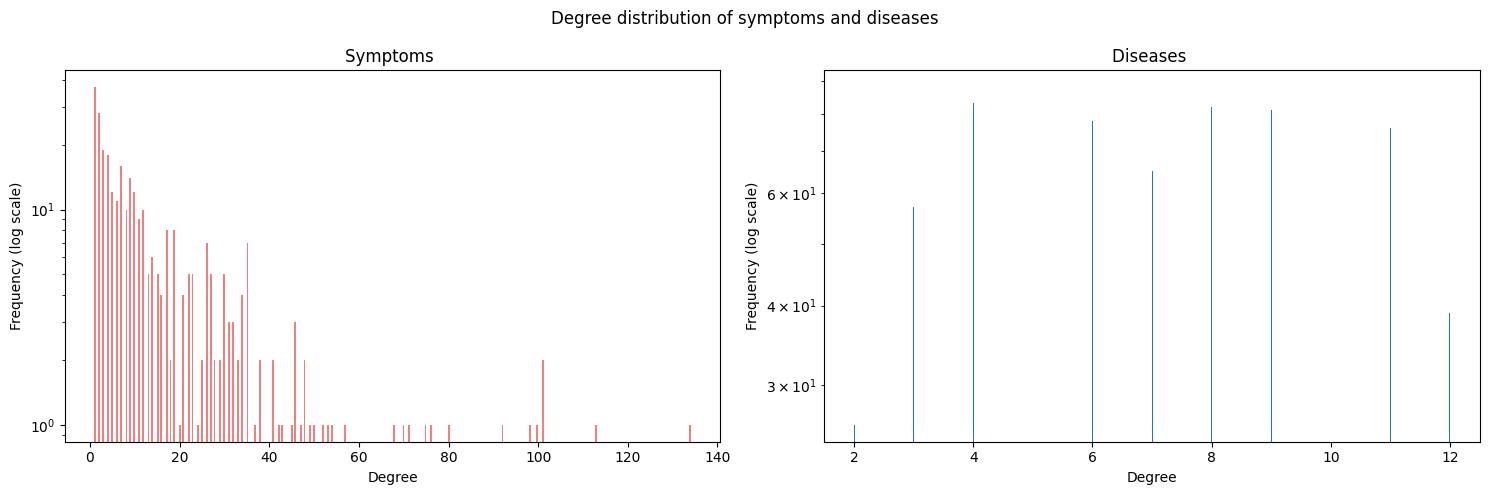
\includegraphics[width=\columnwidth]{degree_distribution.png}
    \caption{Degree Distribution (level 1)}\label{fig:DegreeDistribution}
\end{figure}

\subsubsection*{Level-2 Metrics}
\label{subsubsec:level_2_metrics}
Moving to the level-2 metrics, which capture the interconnectedness and broader impact of symptoms or diseases within the network,
we uncovered intriguing patterns (see Figure~\ref{fig:l2_distribution}).
The Symptom Influence (\textit{SI}) at level-2, reflecting the presence of symptoms across diseases and their associations with other symptoms,
exhibited values ranging from 4 to 12.
This suggests that certain symptoms not only co-occur within diseases but also form meaningful connections with a diverse set of other symptoms.
A higher level-2 Symptom Influence (\textit{SI}) implies a symptom's propensity to be associated with a wide range of symptoms,
indicating its potential impact on various disease pathways.\\
On the other hand, the Disease Influence (\textit{DI}) at level-2, quantifying the ripple effects of a disease's symptoms on other diseases,
demonstrated a wider range, typically spanning from 10 to 80.
This broader range signifies that certain diseases have a more extensive influence on the network by affecting a multitude of other diseases.
A higher level-2 Disease Influence (\textit{DI}) implies that a disease's symptoms not only contribute to its immediate associations
but also have far-reaching consequences, affecting a network of interconnected diseases.\\
These results highlight the diverse roles played by symptoms and diseases in influencing the network when considering higher-order interactions.


\begin{figure}[H]
    \centering
    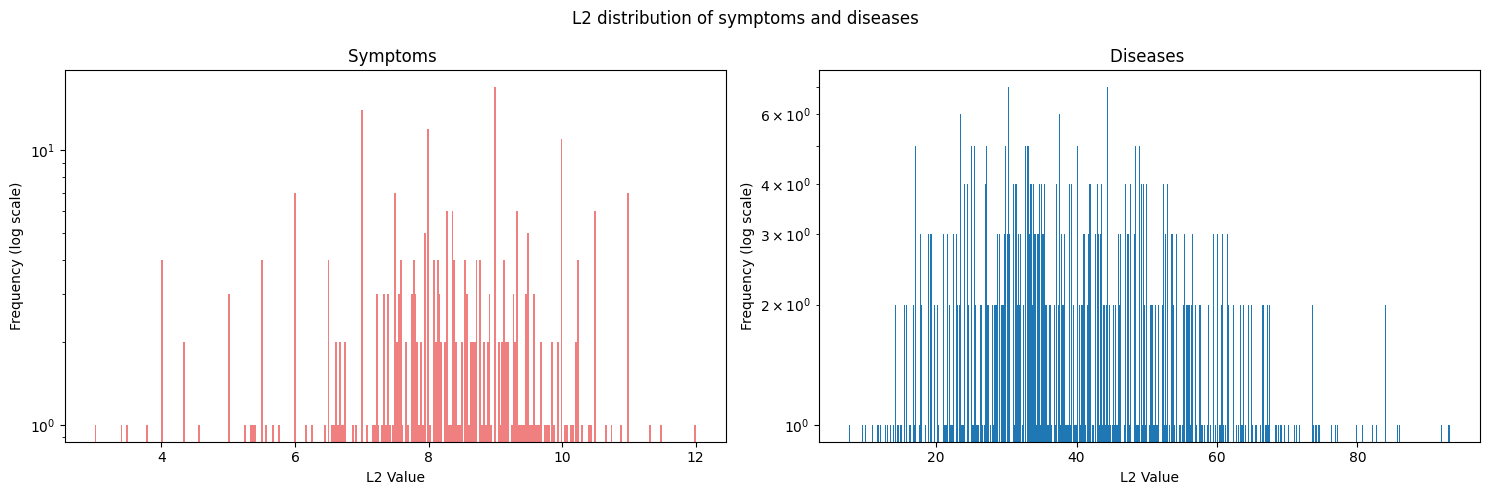
\includegraphics[width=\columnwidth]{L2_distribution.png}
    \caption{L2 Distribution for both symptoms and diseases}\label{fig:l2_distribution}
\end{figure}
\subsubsection*{Power Law CCDF}
\label{subsubsec:power_law_ccdf}


In our statistical validation of the Symptom Influence (\textit{SI}) and Disease Influence (\textit{DI}) indices at both level-1 and level-2,
the analysis of the complementary cumulative probability distribution (CCDF) reveals distinctive patterns.\\
For level-1 diseases, the CCDF power-law behavior exhibits a rapid decrease, indicating that a small number of diseases
have a disproportionately high influence. This steep decline suggests the presence of disease hubs that significantly impact the network dynamics.
Conversely, for level-1 symptoms, the power-law CCDF demonstrates a slow decrease, starting at 0 and extending until 100.
This suggests a more distributed influence of symptoms across diseases, with a considerable number of symptoms exhibiting
varying degrees of prevalence. The gradual decline in the CCDF emphasizes the diverse roles played by symptoms in the network.\\
Level-2 diseases, on the other hand, exhibit a slower power-law decrease, starting at 50 and reaching zero around 90.
This gradual decline implies that a broader range of diseases contributes to the interconnectedness within the network,
with a subset of diseases exerting influence across multiple others.\\
Finally, for level-2 symptoms, the power-law CCDF displays a rapid decrease around 10,
emphasizing the existence of highly influential symptoms that play a pivotal role in connecting various diseases.

\begin{figure}[H]
    \centering
    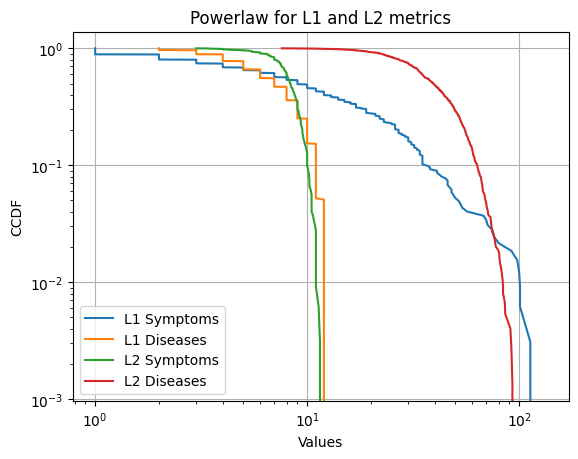
\includegraphics[width=\columnwidth]{powerlaw_hid_metrics.png}
    \caption{Power Law Distribution of the level 1 and level 2 metrics}\label{fig:powerlaw_hid_metrics}
\end{figure}
\subsubsection*{Statistical Validation of SI and DI}

In our statistical validation of the Symptom Influence (\textit{SI}) and Disease Influence (\textit{DI}) indices at level-2,
we aimed to discern whether these higher-order metrics provide additional information compared to level-1,
and whether this information is statistically significant.
Our null hypothesis (\textbf{H0}) posited that level-2 metrics do not offer additional insights beyond level-1,
while the alternative hypothesis (\textbf{H1}) suggested the opposite.\\
Upon generating 5000 random networks with the same level-1 properties as the original network,
we calculated z-scores for both Symptom Influence (\textit{SI}) and Disease Influence (\textit{DI}) at level-2.\\
Remarkably, the z-score distribution (Figure~\ref{fig:pdf_z_score}) for both symptoms and diseases exhibited a shape quite similar to a Gaussian distribution,
with means close to zero.\\
For symptoms, the z-scores ranged between -4 and 3, indicating that the level-2 Symptom Influence (\textit{SI})
values were generally lower than the mean but still within a reasonable range. This suggests that, on average,
symptoms tend to exhibit a level-2 influence that aligns closely with the overall network structure.\\
Similarly, for diseases, the z-scores ranged from -3 to 4, signifying that the level-2 Disease Influence
(\textit{DI}) values were distributed around the mean.
This implies that diseases, on average, have a level-2 influence that aligns with the overall network structure,
showcasing a balance between localized effects and broader impacts.\\
The proximity of the mean to zero in both distributions suggests that, on average,
the level-2 metrics for both symptoms and diseases do not significantly deviate from the null model.
However, the broader range of z-scores signifies the presence of nodes with both positive and negative deviations,
underscoring the heterogeneous nature of influences within the symptom-disease network.\\
In conclusion, our statistical validation reinforces that while the level-2 metrics follow a distribution akin to a Gaussian,
the nuanced deviations reflected by the z-scores
for both symptoms and diseases underscore the diverse and context-dependent nature of their influences within the intricate network structure.

\begin{figure}[H]
    \centering
    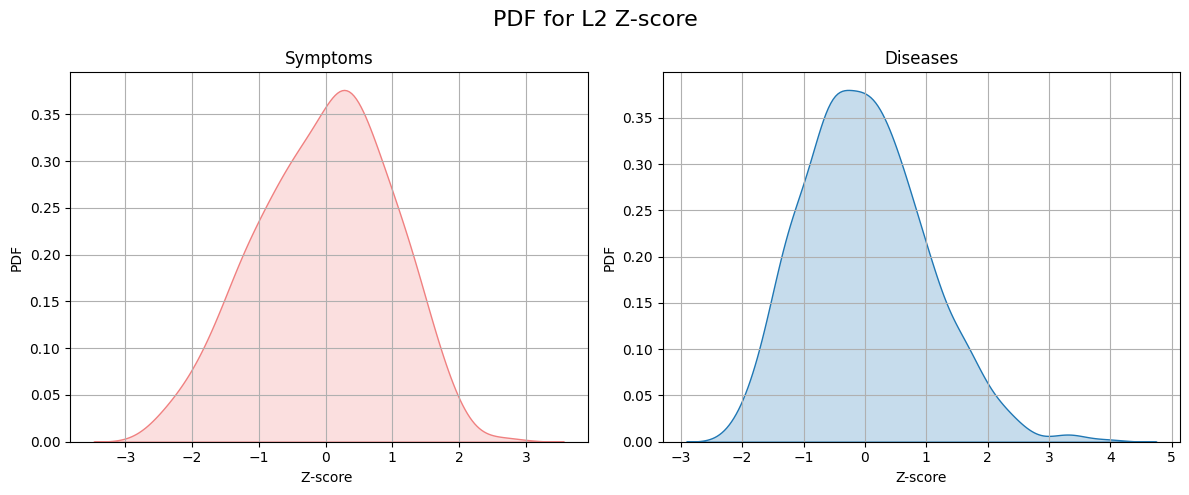
\includegraphics[width=\columnwidth]{PDF_z_score.png}
    \caption{Probability Density Function of the z-scores}\label{fig:pdf_z_score}
\end{figure}
% END: degree distribution and power law

\subsection{Betweenness Centrality}
% BEGIN: betweenness centrality
The examination of betweenness centrality in our bipartite network, as depicted in Figure~\ref{fig:bet_all},
reveals a Power Law Distribution, indicative of a scale-free structure. This implies the presence of a few central
nodes that act as pivotal connectors, while the majority of nodes exhibit lower betweenness centrality.

\begin{figure}[H]
    \centering
    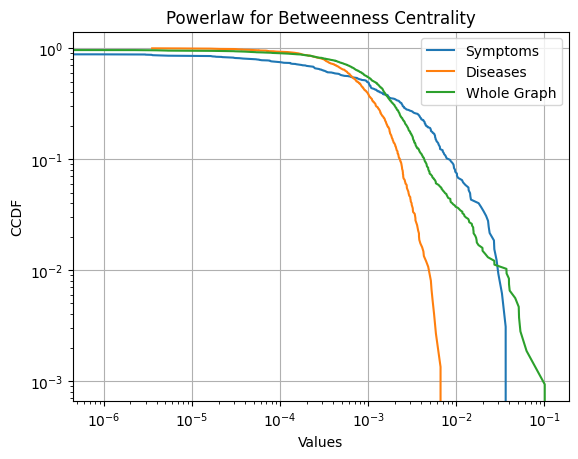
\includegraphics[width=.9\columnwidth]{bet_all.png}
    \caption{Betweenness Centrality CDFs}\label{fig:bet_all}
\end{figure}
\noindent
Upon dissecting the centrality values into symptoms and diseases (see Figures~\ref{fig:bet_diseases} and~\ref{fig:bet_symptoms}),
a notable observation emerges: symptoms tend to have higher betweenness centrality compared to diseases. To decipher the
significance of this result, it's essential to delve into the interpretation of betweenness centrality.

\begin{figure}[H]
    \centering
    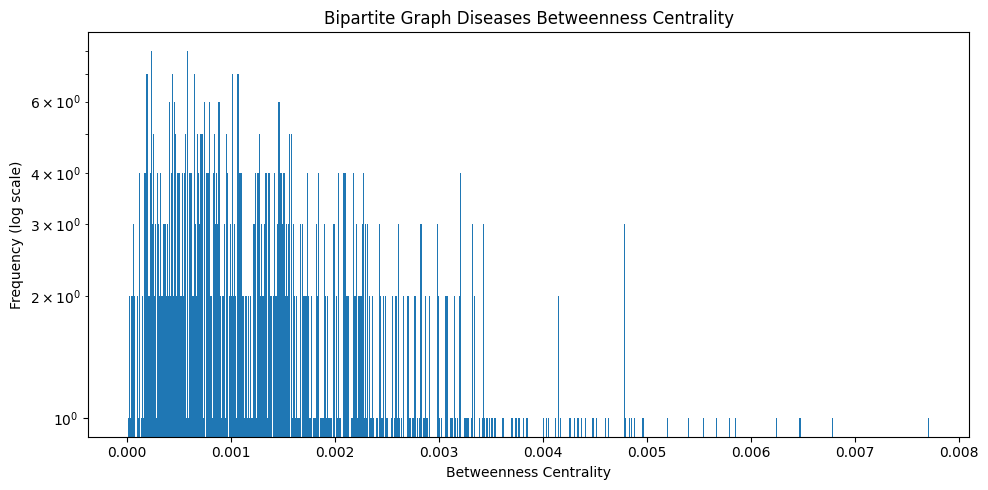
\includegraphics[width=.9\columnwidth]{bet_diseases.png}
    \caption{Betweenness Centrality of the diseases}\label{fig:bet_diseases}
\end{figure}
\noindent
\begin{figure}[H]
    \centering
    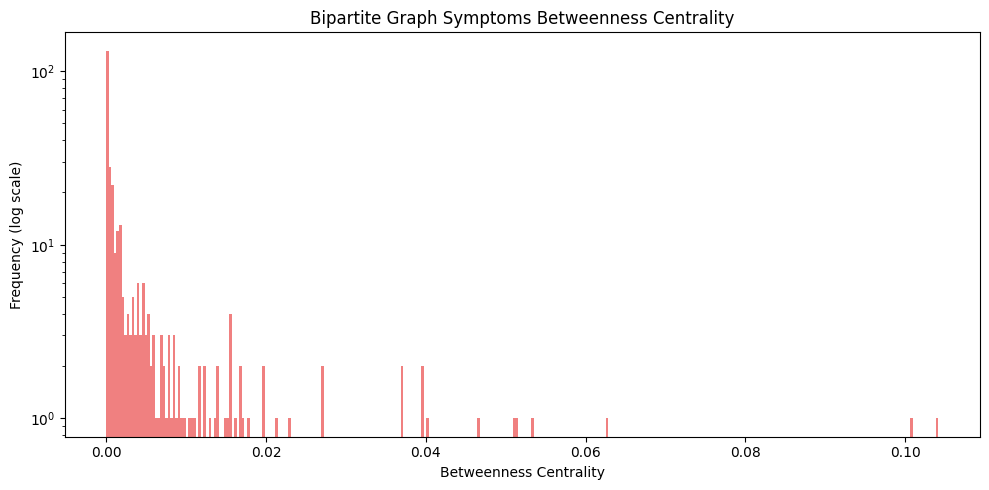
\includegraphics[width=.9\columnwidth]{bet_symptoms.png}
    \caption{Betweenness Centrality of the symptoms}\label{fig:bet_symptoms}
\end{figure}
\noindent
In general, a symptom exhibits high betweenness centrality when it is linked to numerous diseases, and these diseases,
in turn, are connected to a relatively limited set of symptoms. Conversely, a disease attains high betweenness centrality
when it connects to numerous symptoms, and these symptoms are associated with relatively few diseases.\\
Analyzing our results of L1 and L2, it becomes evident that the higher betweenness centrality of symptoms is attributed
to their connections with a multitude of diseases, while diseases, on the contrary, are linked to a relatively limited
number of symptoms. From a predictive standpoint, this outcome may present a challenge as each symptom is not sufficiently
specific, contributing to a broad array of disease classes.\\
Figure~\ref{fig:bet_top} highlights the top 10 nodes with the highest betweenness centrality, all of which are symptoms.
As anticipated, these symptoms are more generic in nature, aligning with their central role in connecting various diseases.

\begin{figure}[H]
    \centering
    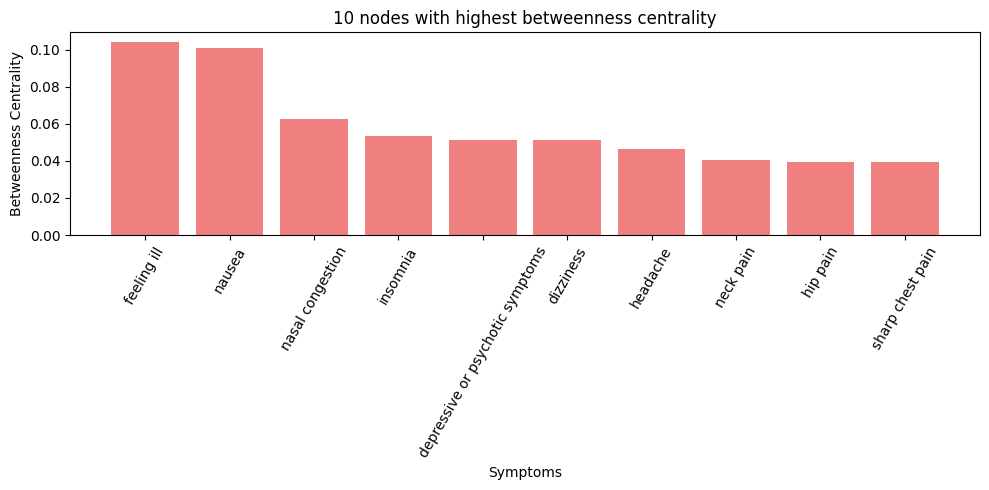
\includegraphics[width=\columnwidth]{bet_top.png}
    \caption{Top 10 nodes with the highest betweenness centrality}\label{fig:bet_top}
\end{figure}
\noindent
% END: betweenness centrality

\subsection{Communities}

% BEGIN: communities
The identification of communities within the network serves a dual purpose – facilitating network interpretation
and enhancing the capabilities of our ML prediction model.\\
From a network interpretation perspective, communities offer insights into disease-symptom relationships.
A community of symptoms signifies a set of symptoms that frequently co-occur within the same diseases, while a
community of diseases identifies a set of diseases often co-occurring within the same symptoms. The sizes of
different communities are illustrated in Figure~\ref{fig:com_sizes_all}.

\begin{figure}[H]
    \centering
    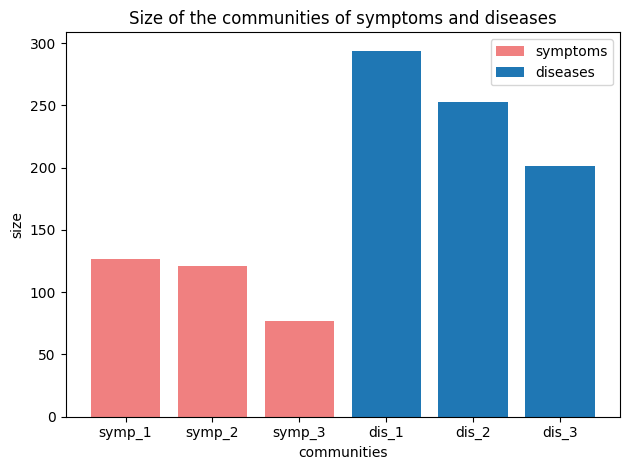
\includegraphics[width=.9\columnwidth]{com_sizes_all.png}
    \caption{Sizes of the communities of symptoms and diseases}\label{fig:com_sizes_all}
\end{figure}

\noindent
For clinical relevance, examining symptoms communities provides valuable information about diseases associated
with these symptoms. This is exemplified in Figures~\ref{fig:com1_symptoms},~\ref{fig:com2_symptoms},
and~\ref{fig:com3_symptoms}. As an example, in the symptoms' community 1 (Figure~\ref{fig:com1_symptoms}),
`burn' has 12 symptoms, which makes it a specific disease for community 1,
considering that on average each disease has only three symptoms from that community.

\begin{figure}[H]
    \centering
    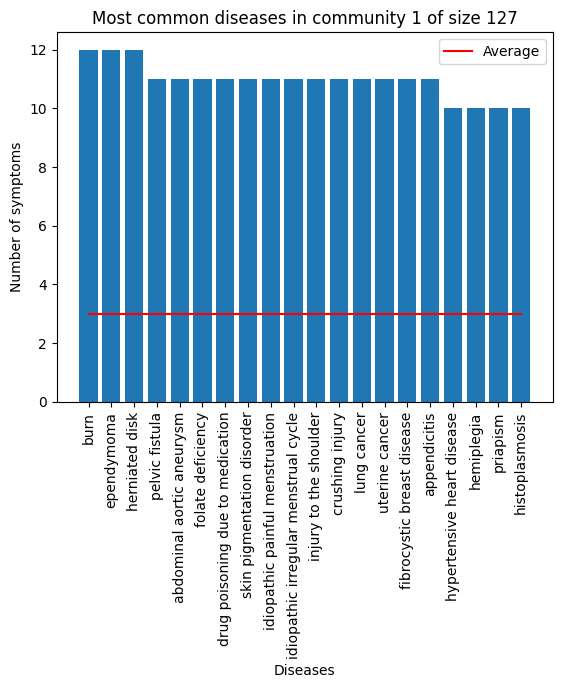
\includegraphics[width=.9\columnwidth]{com1_symptoms.png}
    \caption{Community 1 of symptoms}\label{fig:com1_symptoms}
\end{figure}

\noindent
A similar study can be conducted for communities of diseases, as depicted in Figures~\ref{fig:com1_diseases},
~\ref{fig:com2_diseases},~\ref{fig:com3_diseases}. This information aids in profiling diseases and understanding
the significance of each symptom. For instance, in community 1 of diseases (Figure~\ref{fig:com1_diseases}),
the symptom `sharp abdominal pain' is present in almost half of the diseases in the community, indicating its
generic nature and limited discriminatory value.

\begin{figure}[H]
    \centering
    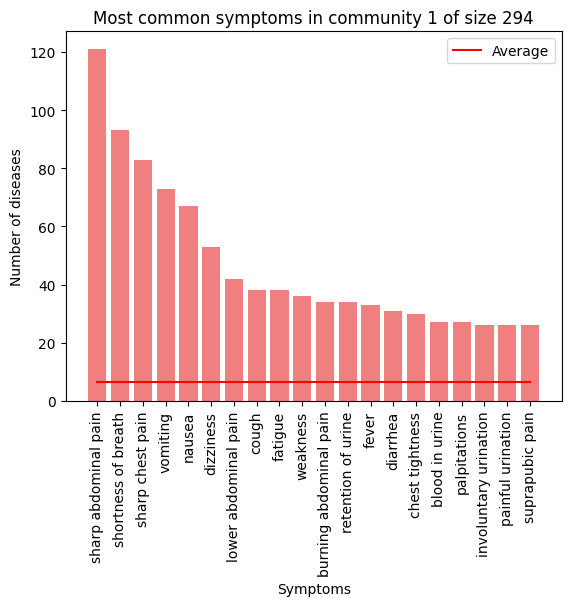
\includegraphics[width=.9\columnwidth]{com1_diseases.png}
    \caption{Community 1 of diseases}\label{fig:com1_diseases}
\end{figure}

\noindent
Transitioning to the creation of features for the ML model, two types of features were developed:\\

\begin{itemize}
    \setlength\itemsep{1em} % set space between items

    \item \textbf{Community Count:} This feature counts how many symptoms of the symptom vector belong to each community.
          Each symptom community is characterized by different pointed diseases. The model can learn to prioritize
          diseases associated with the community with the highest count.

    \item \textbf{Community Size:} This feature replaces each symptom in the symptom vector with the size of the
          community to which the symptom belongs. It enables the model to distinguish between symptoms belonging to small and
          large communities. If many symptoms from small community are present, the associated diseases may be more likely.
\end{itemize}

\noindent
It is noteworthy that communities can also contribute to improving the computational efficiency of the model.
For example, a symptom associated with many diseases may be less informative and could potentially be removed from the
symptom vector. However, we opted for a comprehensive approach using a combination of L1 and L2 measures to address this issue (next section)

% END: communities

\subsection{Most Important Actors}\label{subsec:most_important_actors}
% BEGIN: most important symptoms/diseases (4 classes)

As previously mentioned, our objective extends beyond feature extraction; we aim to leverage network information to
enhance the computational efficiency of the model. The strategy involves reducing the number of symptoms,
retaining only the most significant ones, to decrease training time while maintaining high accuracy.
Various approaches were tested, including L1, L2, betweenness centrality, and the degree of the unipartite projection
of symptoms. To select the most appropriate approach, we examined the correlation between these features
(Figure~\ref{fig:feat_corr}). Indeed, a high correlation between features means that they provide
similar information, and therefore retaining both features would be redundant. On the other hand,
a low correlation between features indicates that they provide complementary information, and this enhances
in a considerable way the quality of the choice.\\
For this reason, as clearly shown in Figure~\ref{fig:feat_corr}, we decided to use L1 and L2 to discriminate
among the symptoms in a more effective manner.

\begin{figure*}[!t]
    \centering
    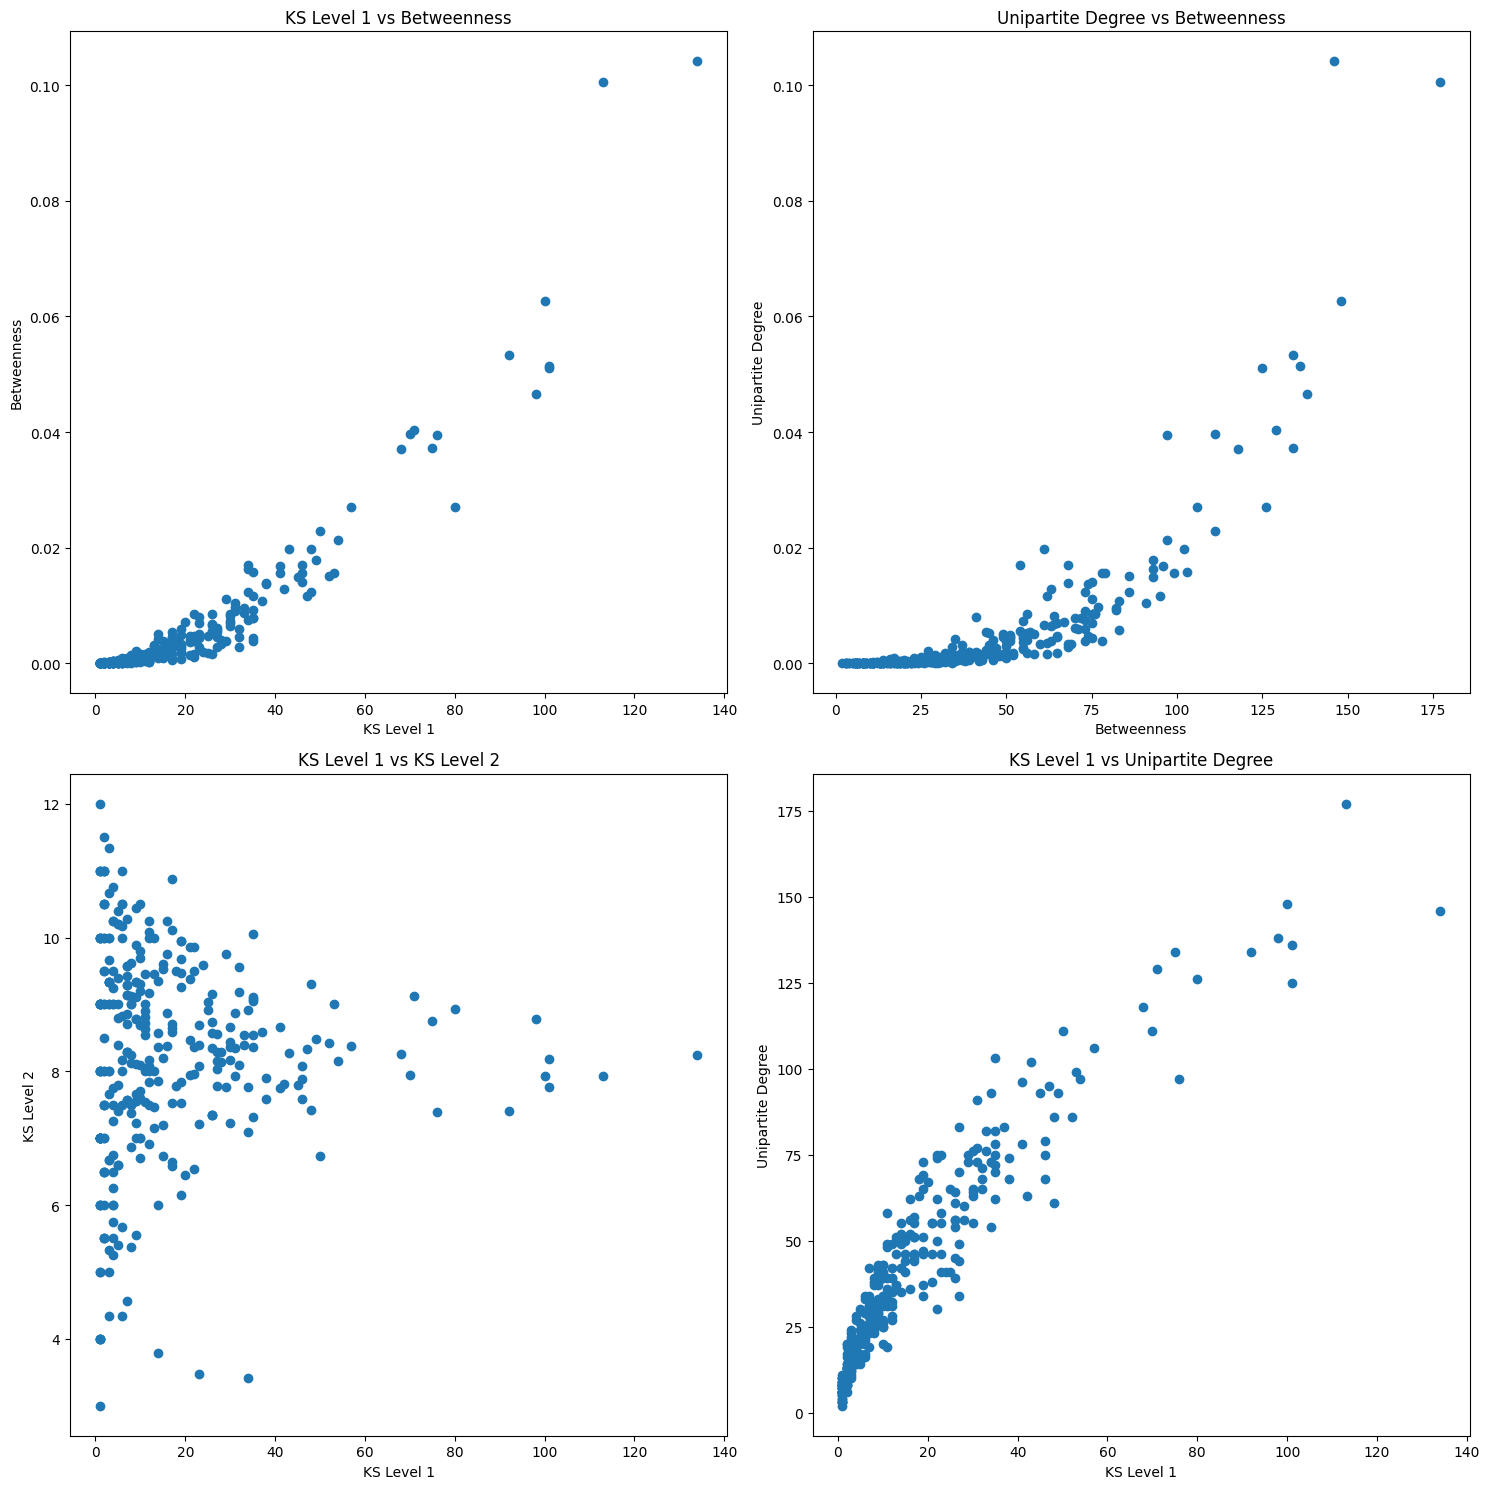
\includegraphics[width=\textwidth]{feat_corr.png}
    \caption{Correlation between features}\label{fig:feat_corr}
\end{figure*}

\noindent
To practically create the classes, we need to define thresholds for L1 and L2. We decided to consider
a symptom as important for the prediction of specific diseases if it is present in less than 0.5 times the average of L1 diseases,
translating into a threshold of 8.21 for L1. Consequently, we adjusted the L2 threshold to maintain a proper balance
between the classes, setting it to 8.

\begin{figure}[H]
    \centering
    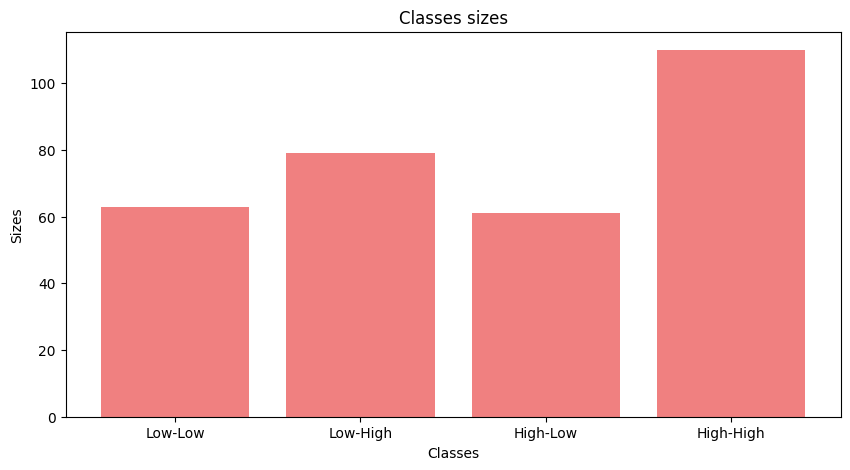
\includegraphics[width=.9\columnwidth]{symptoms_classes.png}
    \caption{Symptoms divided into the four classes}\label{fig:symptoms_classes}
\end{figure}

\begin{figure}[H]
    \centering
    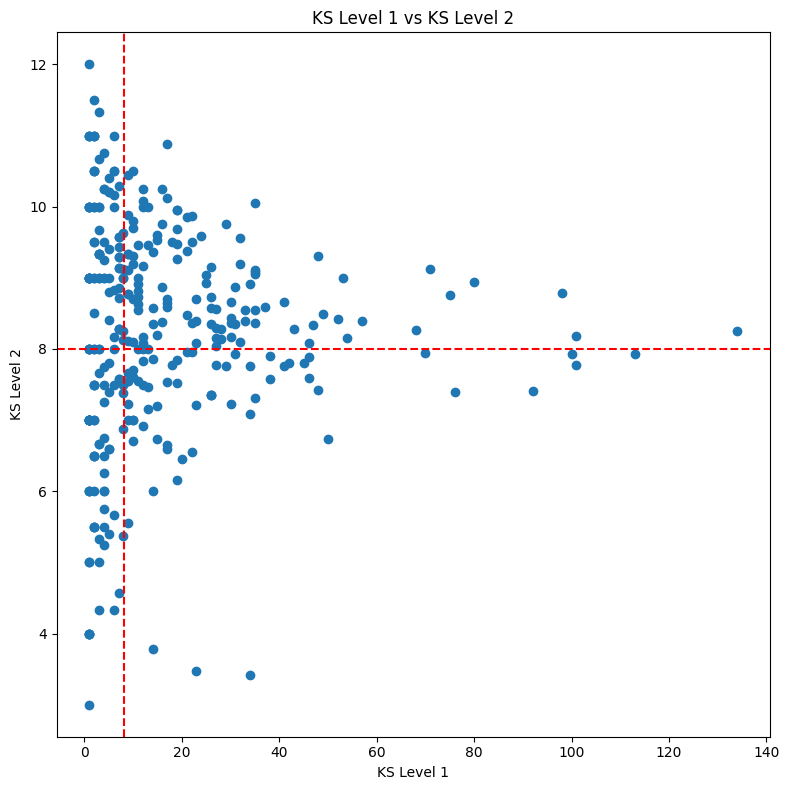
\includegraphics[width=.9\columnwidth]{l1_l2_division.png}
    \caption{Division based on L1 and L2 values}\label{fig:l1_l2_division}
\end{figure}

\noindent
As demonstrated in Figure~\ref{fig:symptoms_classes}, the four classes have different sizes, and more importantly,
they provide very different and valuable information.\\
To shed light on these classes, a brief reminder of the meanings of L1 and L2 is warranted. L1 denotes the number
of diseases associated with a symptom, whereas L2 quantifies the number of symptoms linked to those diseases.
As a result, we categorize the features into the following classes:\\

\begin{itemize}
    \setlength\itemsep{1em}
    \item \textbf{Low L1 - Low L2}: Symptoms with low degree and low L2. These symptoms are connected to few diseases
          which are also connected to few other symptoms. Therefore, we can expect this symptoms to provide a high
          contribution to the prediction of few specific diseases.

    \item \textbf{Low L1 - High L2}: Symptoms with low degree and high L2. For these symptoms, the same reasoning
          as above applies, but with lesser strength. Indeed, these symptoms are connected to few diseases, but those
          diseases are connected to many other symptoms.

    \item \textbf{High L1 - Low L2}: Symptoms with high degree and low L2. These symptoms may be important for the
          overall performance of the model. For instance, a symptom may be associated with many diseases, but those
          diseases may only be associated with that symptom. In this case, the symptom is very important for prediction.
          Since these symptoms are connected to many diseases, they can be considered important for the overall
          performance of the model, even if they are not crucial for the prediction of specific diseases.

    \item \textbf{High L1 - High L2}: Symptoms with high degree and high L2. As for the previous class,
          these symptoms are not very specific of a diseases, but we can expect them to be important for the overall
          accuracy of the model, since they provide information about many diseases.

\end{itemize}

\noindent
As it stands it may not be clear which are the category of symptoms we can get rid of. One can think that the symptoms having bot L1
and L2 low can be the most useful, since they are specific, thus very informative. At the same time the symptoms having both L1 and L2 high
can be the least useful, since a symptom actually appears in many diseases, thus doesn't provide much information.
However we should consider also the model viewpoint. Indeed, if we retain only the symptoms with both L1 and L2 low, we end up
having information about only few diseases, and the model may not be able to learn the patterns of the other diseases, leading
to a poor result in the overall accuracy. To investigate this aspect, once again we adopted a greedy approach, starting from evenly distributed
classes, and starting retaining features from the most promising one. This procedure, whose limits are discussed in
Section \ref{sec:future_works}\ref{subsec:limits}, was applied to the best model and the results are analyzed in
Section \ref{sec:results_ML}\ref{subsec:computational_complexity}.\\
Figures \ref{fig:symptoms_classes} and \ref{fig:l1_l2_division} illustrate the division of symptoms into the four classes.
The same entire analysis was conducted for diseases, in this case focusing on the high-L1-high-L2 class, which contains
the most complex diseases under a symptomatology perspective. The results are reported in Figures \ref{fig:diseases_classes}
and \ref{fig:high_l1_high_l2_class}.\\
To provide a complete picture of the most specific symptoms we report the composition of the low-L1-low-L2 class
in Figure \ref{fig:low_l1_low_l2_class}. As we can see there are many symptoms which occur in just one disease.
Their presence should make their associated diseases the most probable one. As an example, `vulvar sore'
is only present in the diseases `poisoning due to antihypertensives'.\\

\begin{figure*}[!t]
    \centering
    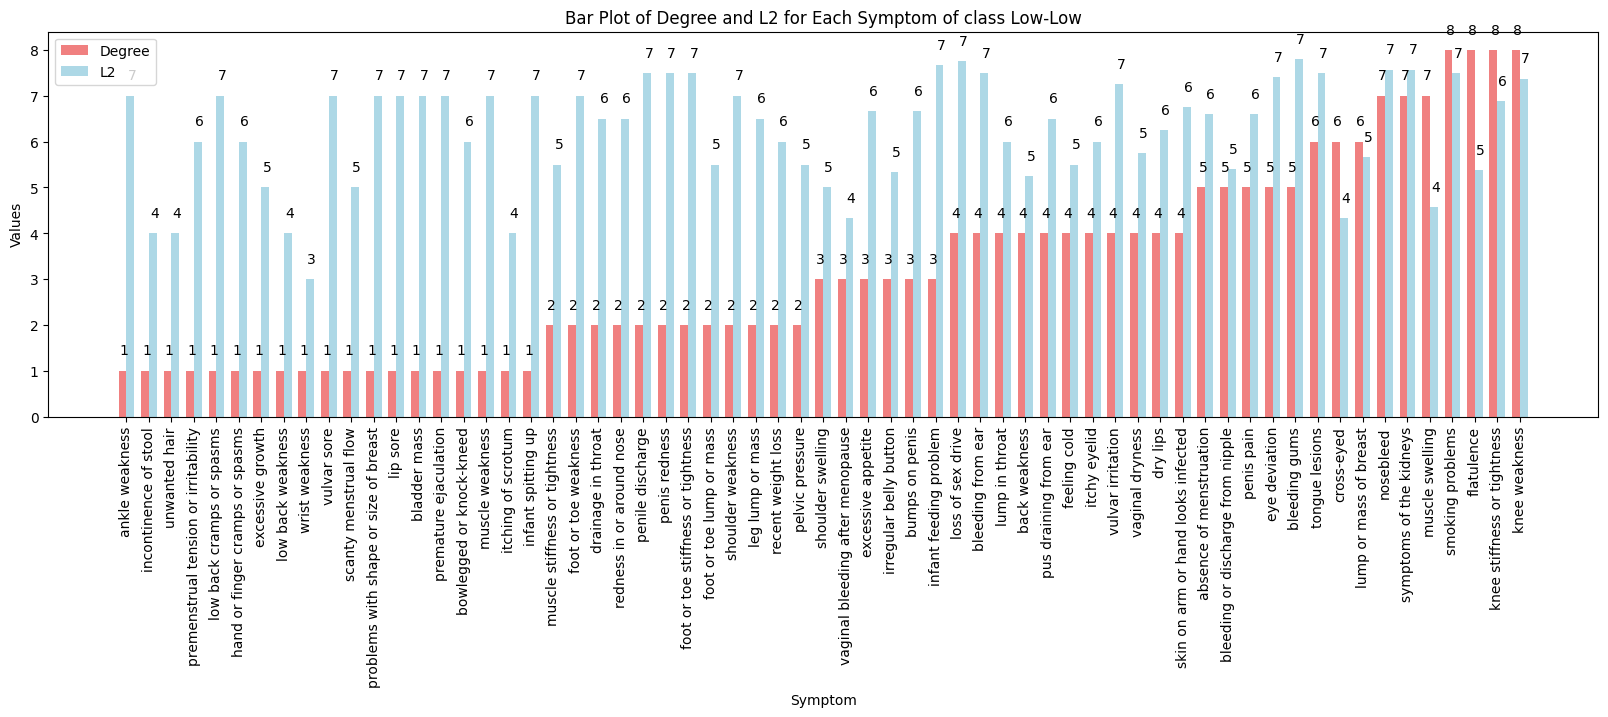
\includegraphics[width=\textwidth]{low_l1_low_l2_class.png}
    \caption{Composition of the low-L1-low-L2 class for symptoms}\label{fig:low_l1_low_l2_class}
\end{figure*}

% END: most important symptoms/diseases (4 classes)






% - degree distribution and power law
% - most important symptoms/diseases (4 classes) 
% - communities
% - L2 has no sense, it's right that z-score low value
% - Meaning of Z-score
% - betweenness centrality
% - clustering coefficient

% ------------------- Methodology and Results ML -------------------

% How we built the ML model 
\section{ML Model Methodology}
\label{sec:methodology_ML}
This section provides a comprehensive overview of the methodologies employed in the construction of the machine
learning model. The discussion encompasses various techniques designed to handle the intricacies of model building,
coupled with a logical flow that guides the entire process.

% ------------------- Data Preparation -------------------

\subsection{Preliminary Data Preparation}\label{subsec:preliminary_data_preparation}
Before delving into model development, a data preprocessing pipeline was employed to properly prepare them for the subsequent steps, facing the problems
of class imbalance and training computational complexity.\\
\begin{itemize}
	\setlength\itemsep{1em} % set space between items
	\item \textbf{Random Sampling}: Given the extensive nature of hyperparameter tuning, we adopted a random sampling strategy, picking around 10\% of the dataset.
	      Instead of training the models on the entire dataset for each hyperparameter combination, the random subset was used to expedite the tuning
	      phase without sacrificing model representativity.
	\item \textbf{Class Imbalance with Oversampling and Undersampling}: The dataset was highly unbalanced across its 700 disease classes.
	      To mitigate this, a combination of oversampling and undersampling techniques was applied. The former was performed for minority classes,
	      while the latter was applied to the majority classes, ensuring all the diseases were adequately represented during training,
	      preventing dominance and biases in the model.
\end{itemize}


% ------------------- Feature Extraction -------------------

\subsection{Feature Extraction}
% - Prepare the features and normalization
A pivotal phase in constructing a machine learning model is feature extraction. In addition to the one-hot vector representation
of symptoms, the network analysis affords us the following features:\\

\begin{itemize}
	\setlength\itemsep{1em} % set space between items
	\item \textbf{L1 and L2 Measures}: A vector with values representing the L1 and L2 measures for each symptom.
	\item \textbf{Betweenness Centrality}: A vector with values denoting the betweenness centrality of each symptom.
	\item \textbf{Community Count}: A vector indicating the number of symptoms belonging to each community.
	\item \textbf{Community Size}: A vector replacing symptoms with the size of the community to which they belong.
\end{itemize}
\noindent
Given the diverse scales of these features, normalization becomes imperative for their cohesive integration into the model
without introducing biases. To achieve this, we opted for \textit{MaxAbs} normalization. This normalization scales each feature
individually, ensuring that the maximal absolute value of each feature in the training set becomes 1.0, while preserving the sparsity of data.


% ------------------- Model Choice -------------------

\subsection{Model Choice}

In the expansive landscape of machine learning, numerous classification models are available for disease prediction.
Our selection narrows down to three models renowned for their robust predictive capabilities,
as substantiated by the findings of \citeauthor{Kohli}~\cite{Kohli}, \citeauthor{Singh}~\cite{Singh}, and \citeauthor{Uddin2019Dec}~\cite{Uddin2019Dec}.
These models are Logistic Regression, Random Forest, and Multilayer Perceptron (MLP).\\

\vspace{0.3cm}
\noindent
\textbf{Logistic Regression}\vspace{0.15cm}\\
Multinomial Logistic Regression, also known as \textit{softmax regression}, extends logistic regression to multi-class classification problems. It models the probability of each class as a function of the input features. The model is given by:

\begin{equation}
	\hat{P}(Y = k | \mathbf{x}) = \frac{e^{\mathbf{w}_k^\top \mathbf{x} + bk}}{\sum_{j=1}^{K} e^{\mathbf{w}_j^\top \mathbf{x} + b_j}}
\end{equation}
\noindent
where $\mathbf{x}$ is the input feature vector, $\mathbf{w}_k$ is the weight vector for class $k$, $b_k$ is the bias term for class $k$, and $K$ is the total number of classes.\\
The output $\hat{P}(Y = k | \mathbf{x})$ is the estimated probability that the input $\mathbf{x}$ belongs to class $k$. The model predicts the class with the highest probability as the output:

\begin{equation}
	\hat{y} = \underset{k}{\arg\max} \left\{ \hat{P}(Y = k | \mathbf{x}) \right\}
\end{equation}
\noindent
Multinomial logistic regression is widely used for classification problems where the output can belong to more than two discrete classes. It is a generalization of binary logistic regression and retains its properties as a linear model, making it interpretable and efficient for high-dimensional datasets.

\begin{itemize}
	\item \textbf{Strengths}: Logistic Regression's computational efficiency makes it an attractive choice for initial exploration and
	      baseline performance assessment. Its simplicity facilitates interpretability, providing insights into the impact of individual symptoms on disease prediction.
	\item \textbf{Considerations}: While efficient, Logistic Regression assumes a linear relationship between features and the
	      log-odds of the target, potentially limiting its ability to capture complex non-linear patterns.
\end{itemize}
\vspace{0.3cm}

\noindent
\textbf{Random Forest}\vspace{0.15cm}\\
A \textit{Random Forest} is an ensemble learning technique used primarily for classification. It constructs a multitude of decision trees during training and integrates their outcomes to improve the final prediction accuracy. The classification decision in a Random Forest is based on the majority voting system among all trees.
The prediction for a class label $\hat{y}$ for an input vector $\mathbf{x}$ is given by:

\begin{equation}
	\hat{y}(\mathbf{x}) = \text{mode} \left\{ T_1(\mathbf{x}), T_2(\mathbf{x}), \ldots, T_B(\mathbf{x}) \right\}
\end{equation}
\noindent
where $B$ is the number of trees in the forest, and $T_b(\mathbf{x})$ is the prediction of the $b^{th}$ tree.
\noindent
The Random Forest algorithm improves classification accuracy by reducing overfitting, a common problem in individual decision trees. This is achieved by creating diversity in the trees through random selection of features and samples, and then aggregating

\begin{itemize}
	\item \textbf{Strengths}: Random Forest is renowned for its robustness in handling large and diverse datasets, making
	      it well-suited for our expansive dataset with 700 disease classes. Moreover, Its ability to capture non-linear relationships
	      ensures that complex patterns within the symptoms' one-hot encoded features are effectively modeled.
	\item \textbf{Considerations}: The ensemble nature of Random Forest provides resilience against overfitting, a crucial factor
	      in the context of disease prediction.
\end{itemize}

\noindent
\vspace{0.3cm}
\textbf{Multilayer Perceptron (MLP)}\vspace{0.15cm}\\
A \textit{Multilayer Perceptron (MLP)} is a type of feedforward artificial neural network, commonly used for classification tasks. It consists of multiple layers of nodes: an input layer, one or more hidden layers, and an output layer. The output of each layer is computed as:

\begin{equation}
	\mathbf{h}^{(l)} = f(\mathbf{W}^{(l)} \mathbf{h}^{(l-1)} + \mathbf{b}^{(l)}) = f(\mathbf{z}^{(l)})
\end{equation}
\noindent
where $\mathbf{h}^{(l)}$ is the output of the $l^{th}$ layer, $\mathbf{W}^{(l)}$ and $\mathbf{b}^{(l)}$ are the weights and biases of the $l^{th}$ layer, respectively, and $f$ is a nonlinear activation function.\\
For classification, the final layer typically uses a softmax activation function to output a probability distribution over the classes. The class with the highest probability is selected as the model's prediction. The softmax function in the output layer for a classification problem with $K$ classes is given by:

\begin{equation}
	\text{softmax}(\mathbf{z})_i = \frac{e^{zi}}{\sum_{k=1}^{K} e^{z_k}} \quad \text{for } i = 1, \ldots, K
\end{equation}
\noindent
where $\mathbf{z}$ is the input to the softmax function, typically the output of the last hidden layer of the network. The final output $\mathbf{y}$ is given by:

\begin{equation}
	\mathbf{y} = \arg\max \left\{ \text{softmax}(\mathbf{z}^{(L)}) \right\}
\end{equation}
\noindent
where $L$ is the total number of layers. The MLP is trained using backpropagation, adjusting its weights and biases to minimize the error in its predictions for the training data.

\begin{itemize}
	\item \textbf{Strengths}: MLPs are adept at capturing intricate relationships in high-dimensional datasets,
	      aligning with the complexity inherent in our 300-feature symptom representation.
	\item \textbf{Considerations}: Their capacity for adapting to non-linear mappings positions MLPs as powerful
	      tools in unraveling the nuanced interactions between symptoms and diseases.
\end{itemize}



% ------------------- Operative Flow -------------------

\subsection{Operative Flow}
% - Operative Flow
% - select best parameters for symptoms one hot only
% - select best parameters for combination of other features (best combination is chosen with random parameters looking at the accuracy)
% - train for each model the two version above with optimal parameters
% - pick the best model according to accuracy
% - train the best model with whole dataset and reduce the number of features

\begin{figure}[t]
	\centering
	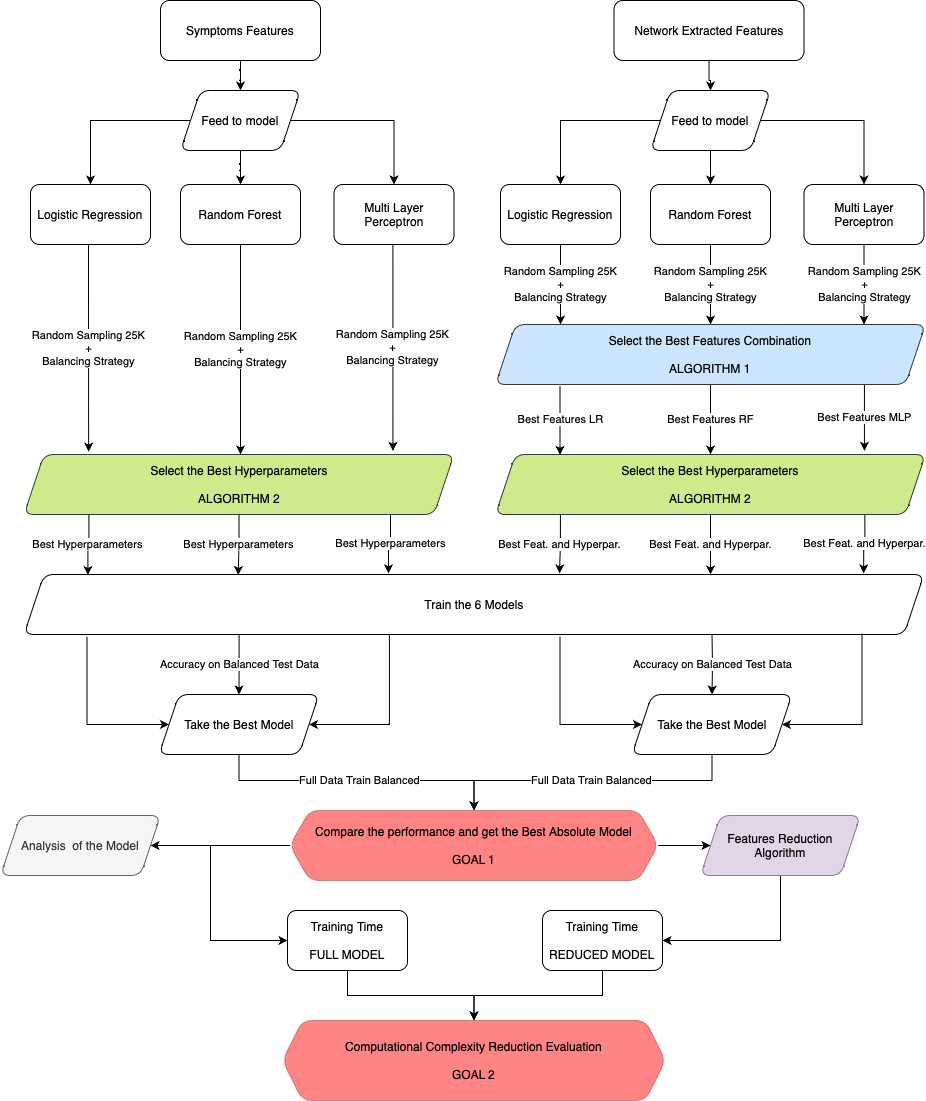
\includegraphics[width=\columnwidth]{operational_flow.png}
	\caption{Operative Flow of the ML Model}\label{fig:ML_operative_flow}
\end{figure}

\noindent
Once the features are ready, the core part of the model-building process can begin. The operational flow was quite complex,
and it is summarized in Figure~\ref{fig:ML_operative_flow}.\\
We trained three different models: a Logistic Regression, a Random Forest, and a Multi-Layer Perceptron (MLP).\\
For each model, we faced the challenge of selecting both the best hyperparameters and the most effective features.
The interdependence between these two aspects makes the optimal approach to explore all the possible combination of features
and for each combination trying all the hyperparameters combination. This approach is not feasible in terms of computational effort
leading us to adopt a greedy approach whose limits are explained in Section \ref{sec:future_works}\ref{subsec:limits}. We firstly split the features into two
groups: the symptoms' one-hot vector and the remaining features. The former is used to train a base model,
while the latter is utilized to explore the potential improvement brought by the new features.\\
Using Algorithm~\ref{alg:feature_selection}, we determined the best feature combination for each group (symptoms and other features).
Subsequently, given the optimal feature combination, we identified the best Hyperparameters combination using Algorithm
~\ref{alg:greedy_hyperparameter_search}. Each model was then trained with the best hyperparameters and the best features combination.
For each group of three models available at this point (3 models with symptoms and 3 models with other features), we selected the best one
according to their accuracy value (Section \ref{sec:results_ML}\ref{subsubsec:results_ML_model_comparison}).
Only at this point the two winning models were trained with the whole dataset to provide a more precise evaluation of their performance and
were compared to assess the result of our first Goal.\\
As regard the last Goal, the best between the above two models undergone the feature reduction process
discussed in Section \ref{sec:results_network}\ref{subsec:most_important_actors} and its computational time was compared to the one of the full features model.\\

\begin{algorithm}[h] \small
	\caption{Feature Selection Algorithm}\label{alg:feature_selection}

	\begin{algorithmic}[1]
		\State RemainingFeatures $\gets$ AllFeatures
		\State FeatureSet $\gets$ EmptySet
		\State BestAccuracies $\gets$ EmptySet
		\State Parameters $\gets$ InitializeRandomParameters
		\State i $\gets$ 0

		\While{RemainingFeatures is not Empty}
		\State BestAccuracy $\gets$ 0

		\For{each feature in RemainingFeatures}
		\State CurrentFeatureSet $\gets$ feature $\cup$ FeatureSet
		\State Model $\gets$ EmptyModel
		\State TrainModel(odel, CurrentFeatureSet, Parameters)
		\State CurrentAccuracy $\gets$ GetAccuracy(Model)

		\If{CurrentAccuracy $>=$ BestAccuracy}
		\State BestAccuracy $\gets$ CurrentAccuracy
		\State BestFeature $\gets$ feature
		\EndIf
		\EndFor

		\State BestAccuracies[i] $\gets$ BestAccuracy
		\State RemainingFeatures $\gets$ RemainingFeatures $-$ BestFeature
		\State FeatureSet $\gets$ BestFeature $\cup$ FeatureSet
		\State BestFeatureCombinations[i] $\gets$ FeatureSet
		\State i $\gets$ i $+$ 1
		\EndWhile
		\State BFC $\gets$ BestFeatureCombinations[ArgMax(BestAccuracies)]
		\State \textbf{return} BFC

	\end{algorithmic}
\end{algorithm}

\noindent
The quest for optimal hyperparameters (hparams) in machine learning models is often constrained by computational resources. In light of these
limitations, we adopted a resource-efficient greedy search strategy to navigate the vast hyperparameter space.
Our approach unfolds in several stages. Initially, we randomly initialize hyperparameters (hparams) to initiate the search. Subsequently, we employ
a stepwise exploration, beginning with the first hyperparameter. For this, we perform an initial search over a small set of values
(e.g., 0.001, 0.01, 1, 10, 100). If the optimum lies at one of the extremes, we extend the search to encompass values in the corresponding
direction.; conversely, if it resides within an intermediate range, we conduct a more focused exploration in a narrower interval.
This process is iteratively repeated for each hyperparameter, gradually refining our understanding of the optimal regions within the
hyperparameter space.
This iterative approach serves a dual purpose. First, it conserves computational resources by avoiding an exhaustive search over all
potential combinations. Second, it capitalizes on the information gleaned from earlier iterations to guide subsequent searches efficiently.
By strategically determining the next set of values based on the observed trends, we strike a balance between exploration and exploitation,
ultimately converging to a set of hyperparameters (hparams) that maximizes model performance. This resource-conscious strategy is paramount when
computational resources are limited, allowing us to derive meaningful results within practical constraints.

% TO BE MODIFIED BY CRISTIAN
\begin{algorithm}[h]
	\caption{Greedy Hyperparameter Search}\label{alg:greedy_hyperparameter_search}
	\begin{algorithmic}[1]
		\State hparams $\gets$ randomInitialization

		\For{each hparam in hparams}
		\State src\_range $\gets$ initialSrcRange
		\State bestVal $\gets$ curr\_hparams[hparam]
		\State accuracy $\gets$ 0

		\For{value in src\_range}
		\State curr\_hparams[hparam] $\gets$ value
		\State performance $\gets$ eval(model, curr\_hparams)

		\If{performance better than accuracy}
		\State bestVal $\gets$ value
		\State accuracy $\gets$ performance
		\EndIf
		\EndFor

		\If{bestVal is at the lower extreme}
		\State src\_range $\gets$ extendSrcRangeLower(bestVal)
		\ElsIf{bestVal is at the upper extreme}
		\State src\_range $\gets$ extendSrcRangeUpper(bestVal)
		\Else
		\State src\_range $\gets$ narrowSrcRange(bestVal)
		\EndIf

		\For{value in src\_range}
		\State curr\_hparams[hparam] $\gets$ value
		\State performance $\gets$ eval(model, curr\_hparams)

		\If{performance better than accuracy}
		\State bestVal $\gets$ value
		\State accuracy $\gets$ performance
		\EndIf
		\EndFor
		\State curr\_hparams[hparam] $\gets$ bestVal
		\EndFor
	\end{algorithmic}
\end{algorithm}

\noindent
At the conclusion of these procedures, we obtained the following two models:\\

\begin{itemize}
	\setlength\itemsep{0.4em} % set space between items
	\item \textbf{Symptoms Model}: The best model with the optimal hparams and the symptoms as features
	\item \textbf{Other Features Model}: The best model with the optimal hyperparameters and the best features combination
\end{itemize}
\vspace{0.4cm}


% - Face the unbalanced dataset problem
% - select best parameters for symptoms one hot only
% - select best parameters for combination of other features (best combination is chosen with random parameters looking at the accuracy)
% - Face the problem of normalization
% - train for each model the two version above with optimal parameters
% - pick the best model according to accuracy

% Results of the ML model (plots and tables)
\section{ML Model Results}\label{sec:results_ML}
In this section we present the results of the ML models we have trained. We then deeply inspect the best performing model,
in order to understand its features and its performance.


% --------------- Model Selection ---------------

\subsection{Model Selection}\label{subsec:results_ML_model_selection}
As previously shown by the operative flow in Figure~\ref{fig:ML_operative_flow}, there are several phases involved in the
selection of the optimal prediction model. Given our limited resources we chose to take a greedy approach by performing
the feature selection first, and then optimizing the hyperparameters at a later time for each of the three models considered.
% MATTEO
% - Matrix plot of stepwise (which is results of algorithm 1) for each model --> to justify the chosen features
\subsubsection*{Features Selection}
To reduce the amount of time spent training the models to select the best hyperparameters, it is best to first limit the
number of features considered. The selection of the most useful features was performed using a forward stepwise selection,
following a greedy a approach that aims at maximizing the accuracy. The hyperparameters were initalized with the default
values provided by the library scikit-learn.\\
As depicted in Figure~\ref{fig:stepwise_acc_logreg}, we can see that the best accuracy with the logistic regression
model is reached after the third iteration, with little improvement with respect to the model using a single feature.
This kind of model seems to favor information about communities and the L2 measure. The feature about the community count is weak on its own,
being the only one that adds 3 columns, but it seems to carry complementary information with respect to the other features,
raising the accuracy by a small margin.
\begin{figure}[h]
	\centering
	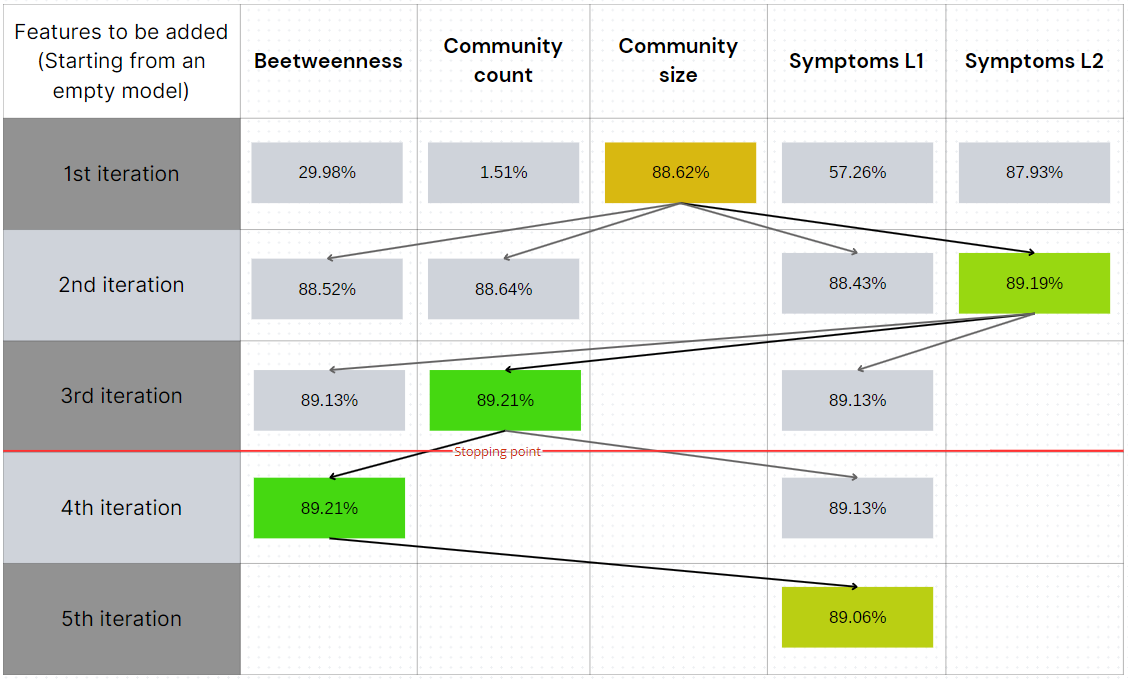
\includegraphics[width=\columnwidth]{stepwise_acc_logreg.png}
	\caption{Accuracy of the logistic regression models over the iterations of the forward stepwise feature selection}\label{fig:stepwise_acc_logreg}
\end{figure}
\noindent
Figure~\ref{fig:stepwise_acc_randomforest} shows that the random forest models work best with less information than logistic regression.
In this case the only features retained are the ones about communities: these results start to reveal which features are the most useful
when it comes to classification.
It is also worth noting that the best random forest model has a slightly worse accuracy than logistic regression,
but that might be due to the random choice of the model's parameters.

\begin{figure}[h]
	\centering
	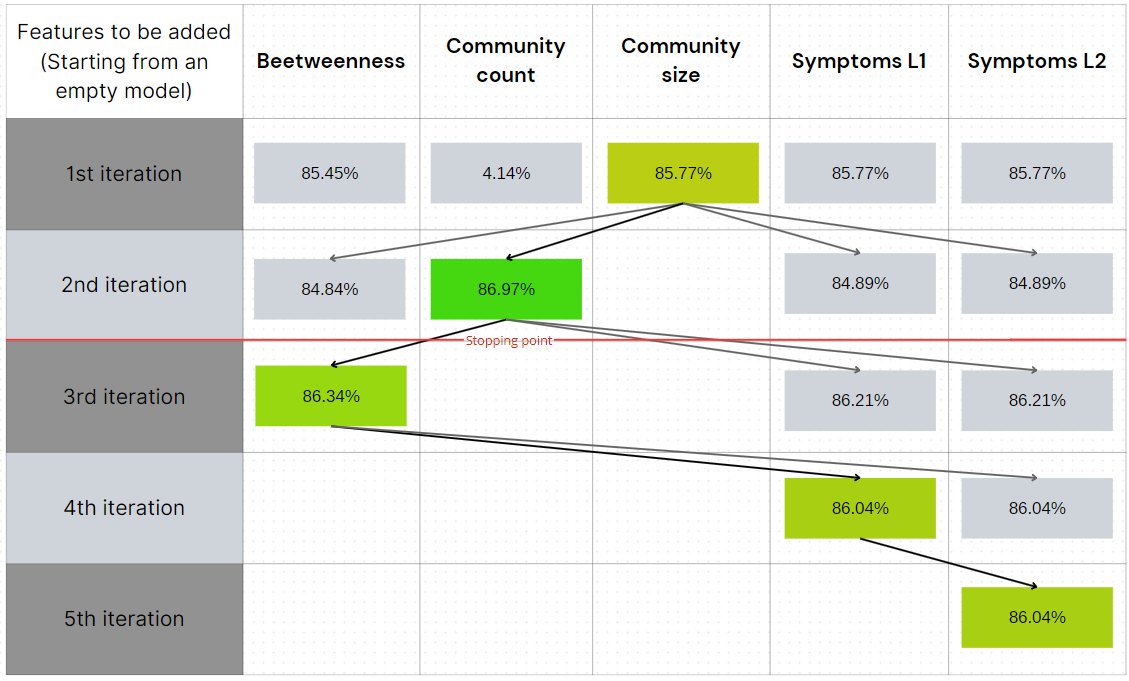
\includegraphics[width=\columnwidth]{stepwise_acc_randomforest.png}
	\caption{Accuracy of the random forest models over the iterations of the stepwise feature selection}\label{fig:stepwise_acc_randomforest}
\end{figure}
\noindent
The multi-layer perceptron model stands in the middle with respect to the other two models in terms of accuracy.
As underlined by Figure~\ref{fig:stepwise_acc_mlp}, unlike the other two cases the model performs its prediction by leveraging only the L2 features,
enhanced by the smaller community count. Two steps are enough to reach the best possible test accuracy.
This particular implementation of neural network has one hidden layer with 100 neurons, and in our case its performance is better
than the random forest model, but still slightly worse than the logistic regression. We expect this to change after the optimization of the hyperparameters,
due to the ability of the MLP to `see' non-linearities.

\begin{figure}[h]
	\centering
	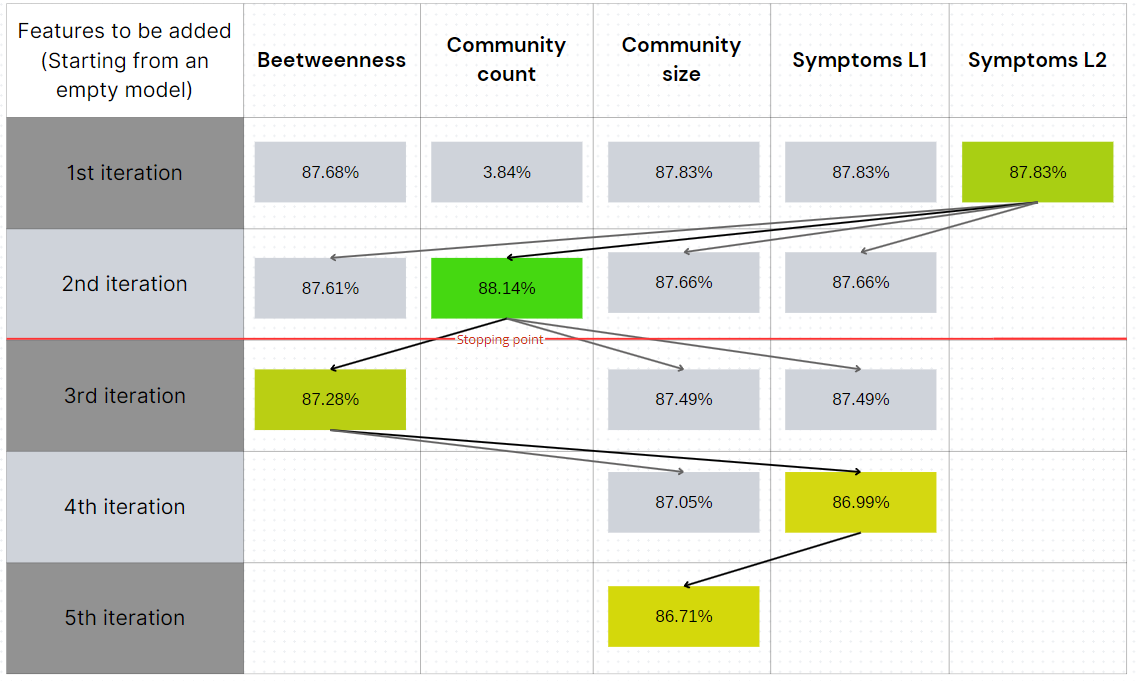
\includegraphics[width=\columnwidth]{stepwise_acc_mlp.png}
	\caption{Accuracy of the MLP models over the iterations of the stepwise feature selection}\label{fig:stepwise_acc_mlp}
\end{figure}

\nocite{Zhang_2016}
% CRISTIAN
% - Comparison for each model of the selected parameters --> to justify the chosen parameters
\subsubsection*{Hyperparameters Selection}

The process of hyperparameter tuning was integral to optimizing the performance of our machine learning models.
We experimented with a range of hyperparameters for each model and identified the best configurations based on test accuracy.
Tables~\ref{logistic_regression_hyperparams},~\ref{random_forest_hyperparams}, and~\ref{mlp_hyperparams} detail the hyperparameters
tested and the best selections for Logistic Regression, Random Forest, and Multi-Layer Perceptron (MLP) respectively.

\rowcolors{2}{blue!8}{blue!18}
\begin{table}[h]
	\centering
	\small
	\begin{tabular}{|c|c|c|}
		\hline
		\textbf{Hyperparameters} & \textbf{Test}                                                                                   & \textbf{Best}                                               \\
		\hline
		C                        & \begin{tabular}[c]{@{}c@{}}0.001, 0.01, 0.1, 0.5,\\ 0.75, 1, 1.25,\\ 1.50, 10, 100\end{tabular} & 1.5                                                         \\
		max iter                 & \begin{tabular}[c]{@{}c@{}}100, 200, 300,\\ 500, 1000\end{tabular}                              & \begin{tabular}[c]{@{}c@{}}Until\\ Convergence\end{tabular} \\
		penalty                  & \begin{tabular}[c]{@{}c@{}}l1, l2,\\ None\end{tabular}                                          & l2                                                          \\
		solver                   & \begin{tabular}[c]{@{}c@{}}lbfgs,\\ liblinear,\\ newton-cg\end{tabular}                         & lbfgs                                                       \\
		\hline
	\end{tabular}
	\caption{Best Hyperparameters for Logistic Regression}
	\label{logistic_regression_hyperparams}
\end{table}

\rowcolors{2}{blue!8}{blue!18}
\begin{table}[h]
	\centering
	\small
	\begin{tabular}{|c|c|c|}
		\hline
		\textbf{Hyperparameters} & \textbf{Test}                                                                    & \textbf{Best} \\
		\hline
		n estimators             & \begin{tabular}[c]{@{}c@{}}50, 80, 100,\\ 200, 300, 400,\\ 500, 600\end{tabular} & 600           \\
		max depth                & \begin{tabular}[c]{@{}c@{}}25, 50, 60,\\ 75, 100, None\end{tabular}              & 50            \\
		min samples split        & \begin{tabular}[c]{@{}c@{}}2, 5,\\ 10, 20\end{tabular}                           & 2             \\
		min samples leaf         & \begin{tabular}[c]{@{}c@{}}1, 2,\\ 5, 10\end{tabular}                            & 1             \\
		\hline
	\end{tabular}
	\caption{Best Hyperparameters for Random Forest}
	\label{random_forest_hyperparams}
\end{table}

\rowcolors{2}{blue!8}{blue!18}
\begin{table}[h]
	\centering
	\small
	\begin{tabular}{|c|c|c|}
		\hline
		\textbf{Hyperparameters} & \textbf{Test}                                                                                                                                                  & \textbf{Best}     \\
		\hline
		First hidden layer       & \begin{tabular}[c]{@{}c@{}} (300)\\ (400)\\(100, 50)\\(500, 200)\\ (60), (80)\\(100), (200)\\ (100, 100, 100)\\ (900, 800, 700)\\ (700, 300, 100)\end{tabular} & (80)              \\
		max iter                 & \begin{tabular}[c]{@{}c@{}}100, 200\\ 300, 500\\ 1000\end{tabular}                                                                                             & Until Convergence \\
		alpha                    & \begin{tabular}[c]{@{}c@{}}0.0001, 0.001\\ 0.01, 0.1, 1\end{tabular}                                                                                           & 0.0001            \\
		activation               & \begin{tabular}[c]{@{}c@{}}relu, tanh\\ logistic, identity\end{tabular}                                                                                        & relu              \\
		\hline
	\end{tabular}
	\caption{Best Hyperparameters for MLP}
	\label{mlp_hyperparams}
\end{table}
\noindent
These hyperparameter configurations were carefully selected to maximize the performance of each model. The Logistic Regression model, with its optimal C value and penalty type, demonstrates a balance between model complexity and regularization. The Random Forest model's parameters, such as the number of estimators and maximum depth, were chosen to balance the bias-variance trade-off, ensuring robustness and generalization. Lastly, the MLP model, with its specific hidden layer sizes and activation function, was configured to effectively capture complex, non-linear relationships in the data.


% ANDREA
% - Comparison of the three models with best combination of features and best parameters
% - precision, recall, AUC, accuracy
\subsubsection*{Model Comparison}\label{subsubsec:results_ML_model_comparison}

As illustrated in Figure~\ref{fig:ML_operative_flow}, our model ensemble now comprises six variants:
three leveraging only symptoms and three incorporating new network-based features. The selection of
the best-performing model from each group was based on test accuracy assessment, where the test is the same balanced dataset
in all cases. Figure~\ref{fig:acc_symptoms}
illustrates consistently low overfitting across all models, showcasing the stability of the symptom-only
models. In contrast, Figure~\ref{fig:acc_new_features}, portraying the accuracy of models with the new
features, reveals some overfitting, particularly in the MLP and Random Forest.\\
The observed tendency for models with new features to exhibit more pronounced overfitting is unsurprising,
given the greater number and complexity of these features compared to symptoms. Notably, despite their different
complexity, all models demonstrate similar test accuracy levels, suggesting that a linear separation
boundary suffices for effective feature classification. Considering this, we retain the Logistic Regression
model as the best-performing model in each group, striking a balance between performance and complexity.

\begin{figure}[h]
	\centering
	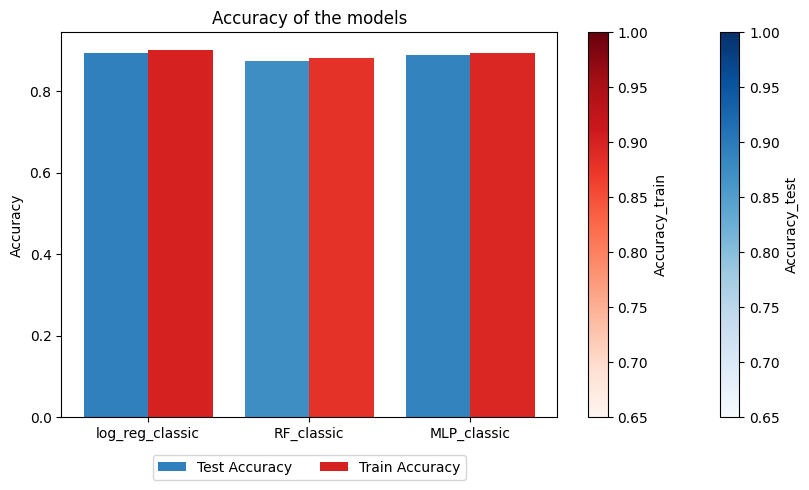
\includegraphics[width=\columnwidth]{acc_symptoms.png}
	\caption{Accuracy of the three models with only symptoms}\label{fig:acc_symptoms}
\end{figure}

\begin{figure}[h]
	\centering
	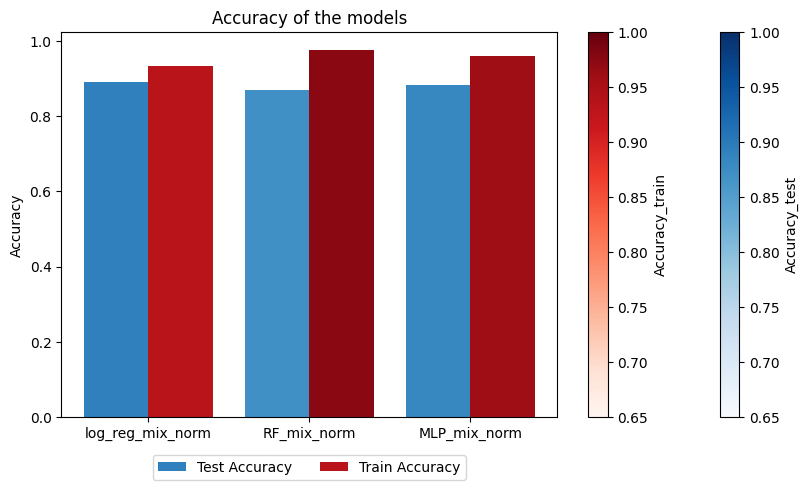
\includegraphics[width=\columnwidth]{acc_new_features.png}
	\caption{Accuracy of the three models with new features}\label{fig:acc_new_features}
\end{figure}



% --------------- New Features Effect ---------------

\subsection{New Features Effect}
% ANDREA
% - compare the best symptoms one hot model with the best one with the new features

\noindent
The best model from each group was further trained on the full balanced dataset to ensure a more reliable
performance evaluation and the test accuracy was computed on the real unbalanced data.
The results in Figure~\ref{fig:acc_best_models} reveal a minimal difference between
the two groups. This addresses our \textbf{first goal}: the new features, only slightly improve the model,
offering a comparable performance to using symptoms alone. However, It's essential to note that the new features are
more numerous than the symptoms, contributing to a more complex model. In conclusion, the extracted network
features are not a superior alternative to symptoms.\\
It is worth to underline that the `simplicity' of the dataset, which leads to a very high accuracy in all models, may also affect the performance
evaluation of the new features, which have a small room to improve the model. Therefore, a possible avenue
for future exploration could involve the use of more complex dataset, to better assess the performance of the
new features.\\
Another viable option for future work is to use the new features as a complement to the symptoms.


% THE FIGURE IS THE FIGURE OF MODEL FULLY TRAINED ON THE BALANCED DATASET


\begin{figure}[h]
	\centering
	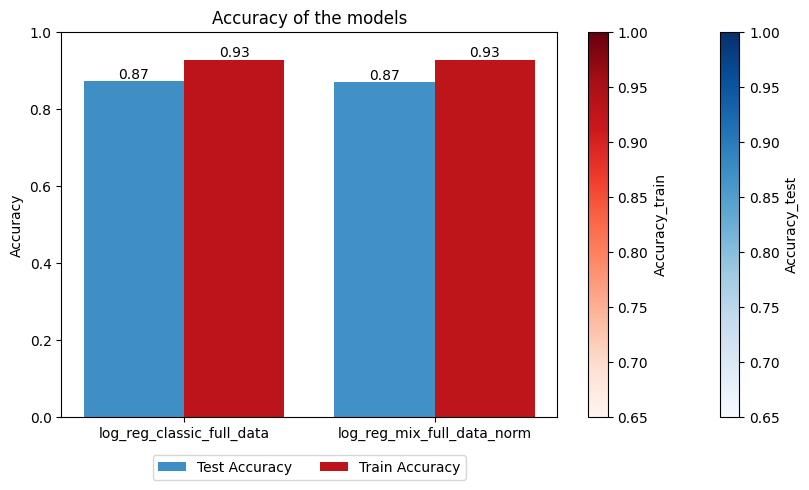
\includegraphics[width=\columnwidth]{acc_best_models.png}
	\caption{Accuracy of the best models from both groups}\label{fig:acc_best_models}
\end{figure}



% --------------- Best Model Performance ---------------

\subsection{Best Model Analysis}
Given that the logistic regression using only symptoms and the one with the new features achieve the same accuracy,
we have selected the logistic regression with the new features as the superior model for further analysis.
Considering its greater complexity and the small level of overfitting,
this model has the potential to capture more nuanced information and intricate patterns.\\
The model contains 3 group of features: community size, SI index level 2 and community count.
\subsubsection*{Performance analysis}
The performance of our predictive model, as demonstrated by the confusion matrix in Figure \ref{fig:conf_matrix},
is indicative of its capability to effectively distinguish between different disease classes.
These classes are stratified based on their respective Disease Influence (DI) indices.

\begin{itemize}
	\item \textbf{Class 1: Low DI L1 - Low DI L2:} Diseases with a low degree (DI L1) and their symptoms are connected to a limited number
	      of other diseases (DI L2) tend to be highly specific, which is reflected in the model's precision for such cases.
	      The confusion matrix exhibits a low misclassification rate for these diseases,
	      suggesting that when such specific symptoms are presented, the model can predict with high confidence,
	      albeit for a restricted number of cases.

	\item \textbf{Class 2: Low DI L1 - High DI L2:} Diseases characterized by a low DI L1 but a high DI L2 are connected to a few symptoms,
	      which in turn are associated with a wider array of other diseases. The model's performance for these diseases,
	      as shown in the confusion matrix, presents a moderate degree of accuracy.
	      Misclassifications may occur due to the broader symptom overlap with other diseases.

	\item \textbf{Class 3: High DI L1 - Low DI L2:} A high DI L1 coupled with a low DI L2 signifies diseases with numerous related symptoms,
	      which however, do not significantly influence other diseases.
	      The confusion matrix suggests that such diseases are predicted with a considerable degree of accuracy.
	      The symptoms, while not disease-specific, contribute to a heightened overall model performance due to their prevalence.

	\item \textbf{Class 4: High DI L1 - High DI L2:} Diseases with both high DI L1 and DI L2 indices are those that exhibit common symptoms
	      influencing a multitude of other diseases. The confusion matrix shows that the model is generally accurate in predicting these diseases.
	      However, due to the commonality of symptoms, there is an inherent challenge in precisely classifying them,
	      which could result in a higher misclassification rate with diseases sharing similar symptom profiles.
\end{itemize}
\noindent
The aforementioned analysis underscores the complexity inherent in disease-symptom relationships and their impact on predictive modeling.
As the confusion matrix corroborates, our model adeptly handles diseases with distinct symptom profiles (Low DI L1 - Low DI L2)
but is challenged by diseases sharing common symptoms (High DI L1 - High DI L2).
Consequently, the model's performance is a direct reflection of the nuanced interplay between disease prevalence and symptom specificity,
as encapsulated by the DI indices.
\begin{figure}[h]
	\centering
	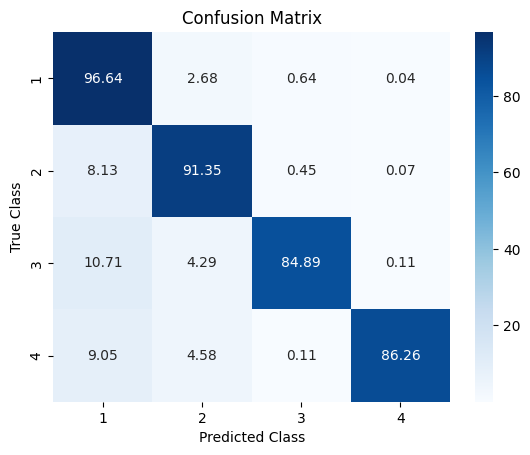
\includegraphics[width=\columnwidth]{conf_matrix_best_model.png}
	\caption{Confusion matrix of the predictive model}\label{fig:conf_matrix}
\end{figure}
\noindent
Figure~\ref{fig:performance_graph} displays a detailed comparison of the model's diagnostic efficacy for a wide range of diseases,
identified by their numerical codes on the x-axis.
The graph features two key metrics: the F1 score and accuracy, represented by blue and orange lines, respectively.
The accuracy line, mostly stable and high, shows the model's consistent ability to correctly detect both presence and absence of each disease.
In contrast, the F1 score line, more varied, reflects the complexity and variability in predicting disease symptoms,
illustrating the model's precision and recall for each disease. High points on the F1 score indicate optimal model performance,
with a balanced precision and recall, effectively identifying true disease cases without errors.
Low points, however, highlight areas where the model is less effective.
\begin{figure*}[htbp]
	\centering
	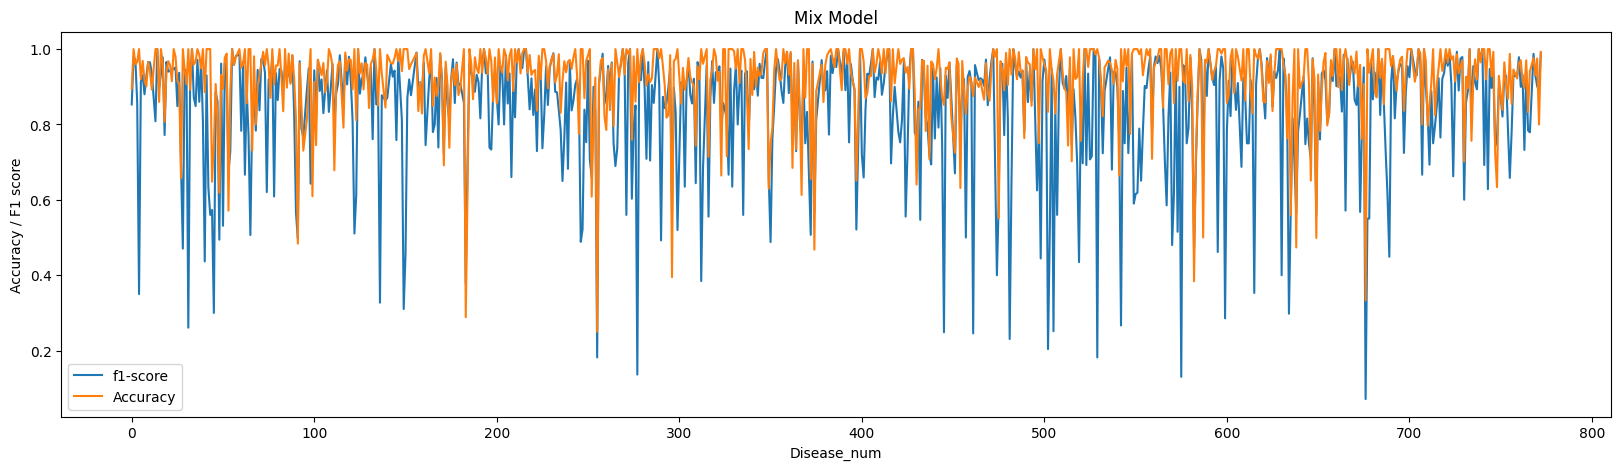
\includegraphics[width=.8\textwidth]{accuraci_diseases_best_model.png}
	\caption{A comparison of the F1 score and accuracy for each disease predicted by the model.}
	\label{fig:performance_graph}
\end{figure*}
\subsubsection*{Best and worst performing diseases}
Our diagnostic model's effectiveness is analyzed by assessing its performance across different diseases.\\
Table~\ref{best} lists the top ten diseases where the model demonstrates high accuracy.
This exceptional performance is further highlighted by near-perfect f1-scores, indicating an optimal balance of precision and recall.
Diseases like mitral valve disease, syndrome of inappropriate secretion, and acute bronchospasm stand out with f1-scores of 1.0,
exemplifying the model's precision in diagnosing these conditions without any errors.\\
On the other hand, Table~\ref{worst} outlines the ten diseases with the lowest accuracy,
indicating areas where the model's diagnostic efficiency is limited. While accuracy is lower for these diseases,
the f1-scores for conditions like premature ventricular contractions and histoplasmosis reveal that the model,
when accurate, maintains reasonable precision and recall.
Nevertheless, the notable decline in f1-score for ailments such as vitamin b12 deficiency and otitis media reveals a significant imbalance
in the model's diagnostic precision and recall, underscoring the need for targeted improvements in these specific areas.
\rowcolors{2}{green!8}{green!18}
\begin{table}[H]
	\centering
	\small
	\begin{tabular}{|c|c|c|}
		\hline
		\textbf{Disease}                    & \textbf{Accuracy} & \textbf{f1-score} \\
		\hline
		mitral valve disease                & 1.0               & 1.000000          \\
		syndrome of inappropriate secretion & 1.0               & 1.000000          \\
		acute bronchospasm                  & 1.0               & 1.000000          \\
		eye alignment disorder              & 1.0               & 1.000000          \\
		reactive arthritis                  & 1.0               & 1.000000          \\
		joint effusion                      & 1.0               & 0.985507          \\
		anal fistula                        & 1.0               & 0.823529          \\
		open wound of the shoulder          & 1.0               & 0.791667          \\
		alzheimer disease                   & 1.0               & 0.769231          \\
		infectious gastroenteritis          & 1.0               & 0.666667          \\
		\hline
	\end{tabular}
	\caption{Accuracy and f1 score for the 10 diseases with the highest accuracy}
	\label{best}
\end{table}


\rowcolors{2}{red!8}{red!18}
\begin{table}[H]
	\centering
	\small
	\begin{tabular}{|c|c|c|}
		\hline
		\textbf{Disease}                     & \textbf{Accuracy} & \textbf{f1-score} \\
		\hline
		premature ventricular contractions   & 0.500000          & 0.666667          \\
		histoplasmosis                       & 0.498876          & 0.560252          \\
		hemiplegia                           & 0.483908          & 0.496462          \\
		acute bronchiolitis                  & 0.473684          & 0.562500          \\
		poisoning due to antimicrobial drugs & 0.467849          & 0.567968          \\
		open wound of the mouth              & 0.394890          & 0.564315          \\
		acute otitis media                   & 0.383938          & 0.468456          \\
		vitamin b12 deficiency               & 0.333333          & 0.071429          \\
		bladder cancer                       & 0.288740          & 0.378102          \\
		otitis media                         & 0.250000          & 0.181818          \\
		\hline
	\end{tabular}
	\caption{Accuracy and f1 score for the 10 diseases with the lowest accuracy}
	\label{worst}
\end{table}

\subsubsection*{Analysis of bladder cancer}

Bladder cancer, as identified in Table~\ref{worst}, is a disease with notably low diagnostic accuracy in our model,
prompting a more detailed investigation. Figure~\ref{fig:cancer_missclassified}
illustrates the proportion of bladder cancer cases incorrectly identified by the model, revealing frequent misclassifications,
especially as diabetes insipidus and hemiplegia.\\
Figures~\ref{fig:cancer_diabet} and~\ref{fig:caner_hemiplegia} delve deeper, showing the number of bladder cancer cases exhibiting
symptoms akin to diabetes insipidus and hemiplegia, respectively. It's striking that 90\% of bladder cancer samples share
symptoms with diabetes insipidus and hemiplegia, clarifying why the model often confuses bladder cancer with these diseases.\\
Moreover, an important factor contributing to this diagnostic challenge is the representation of bladder cancer in our dataset.
Constituting only 0.36\% of the total data, this limited presence may significantly impact the model's ability to accurately identify bladder cancer,
leading to its lower accuracy for this specific condition.
\begin{figure*}[htbp]
	\centering
	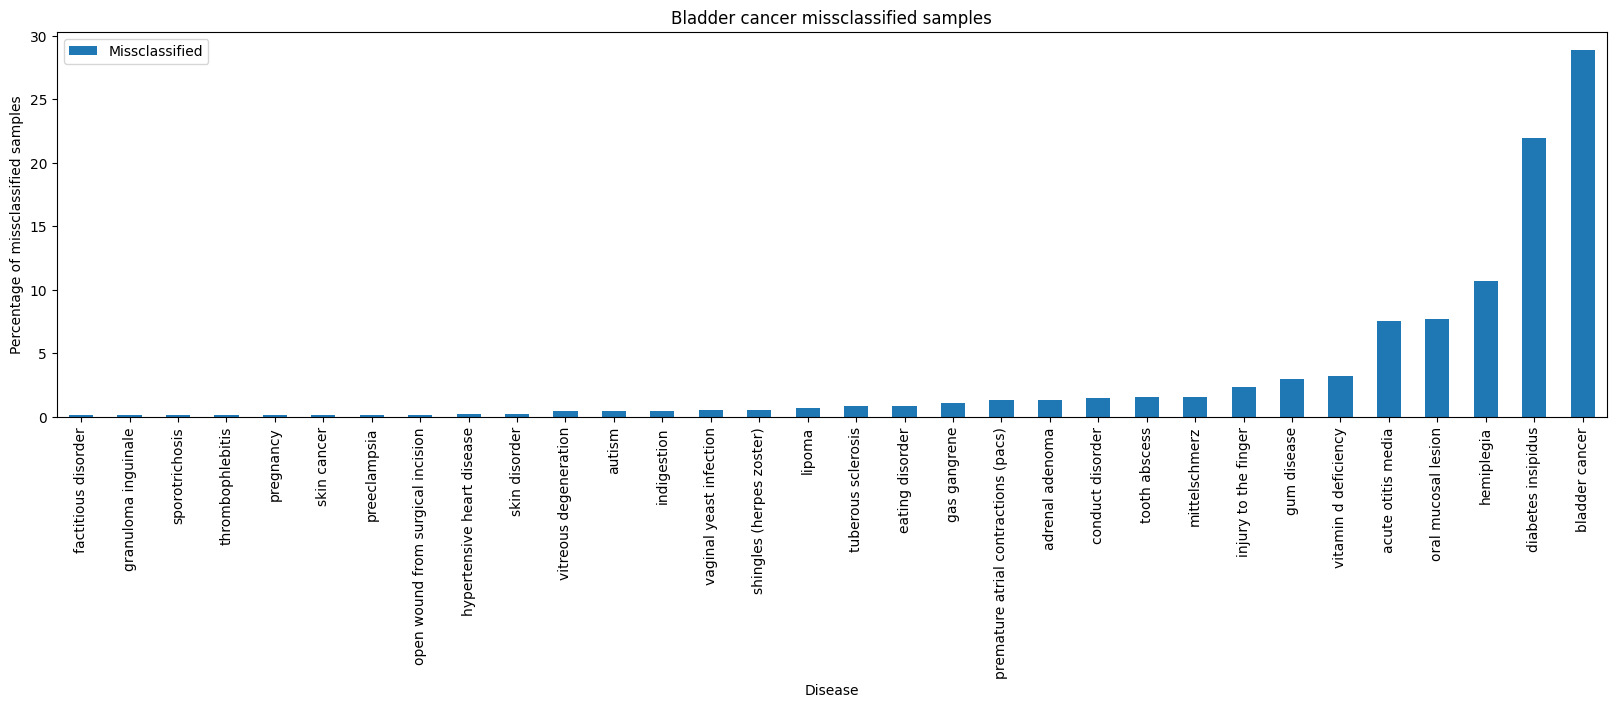
\includegraphics[width=\textwidth]{bladder_cancer_missclassified.png}
	\caption{Percentage of bladder cancer samples misclassified}\label{fig:cancer_missclassified}
\end{figure*}
\noindent

\begin{figure}[H]
	\centering
	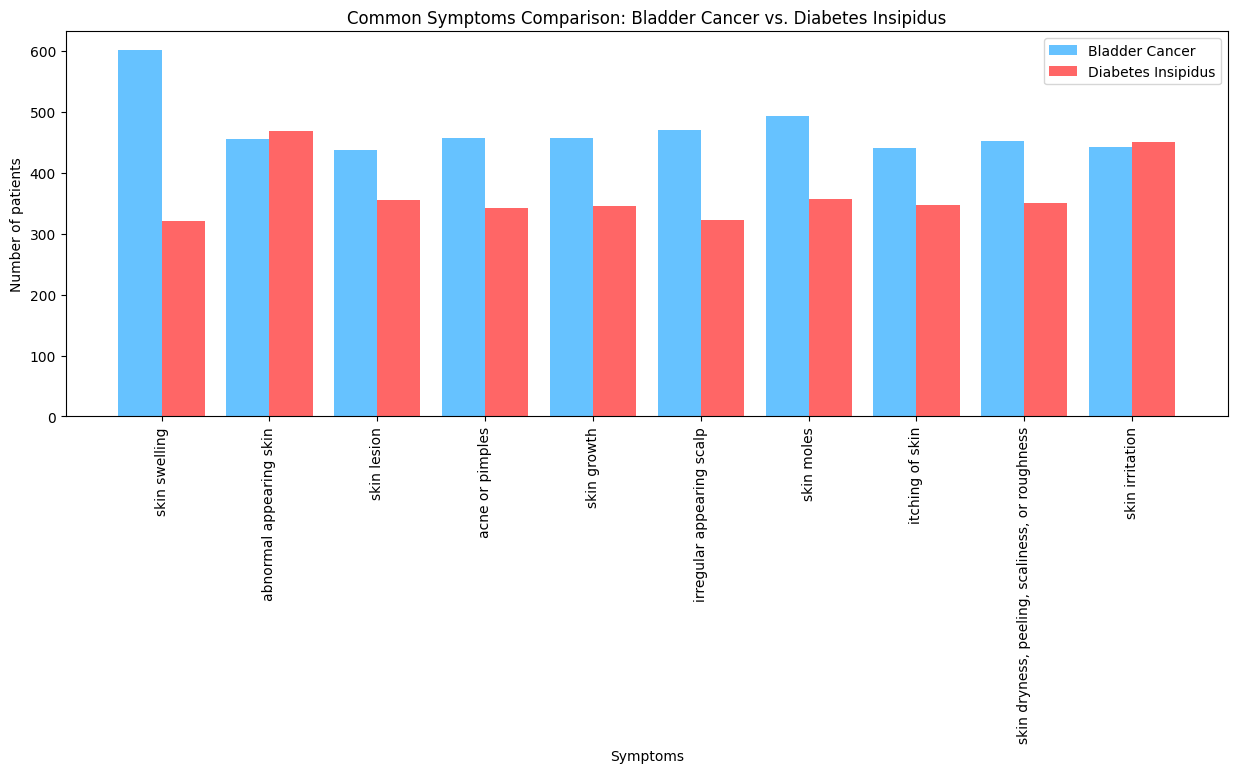
\includegraphics[width=\columnwidth]{cancer_diabet}
	\caption{number of samples of bladder cancer and diabets insipidus that have the same symptoms}\label{fig:cancer_diabet}
\end{figure}
\noindent

\begin{figure}[H]
	\centering
	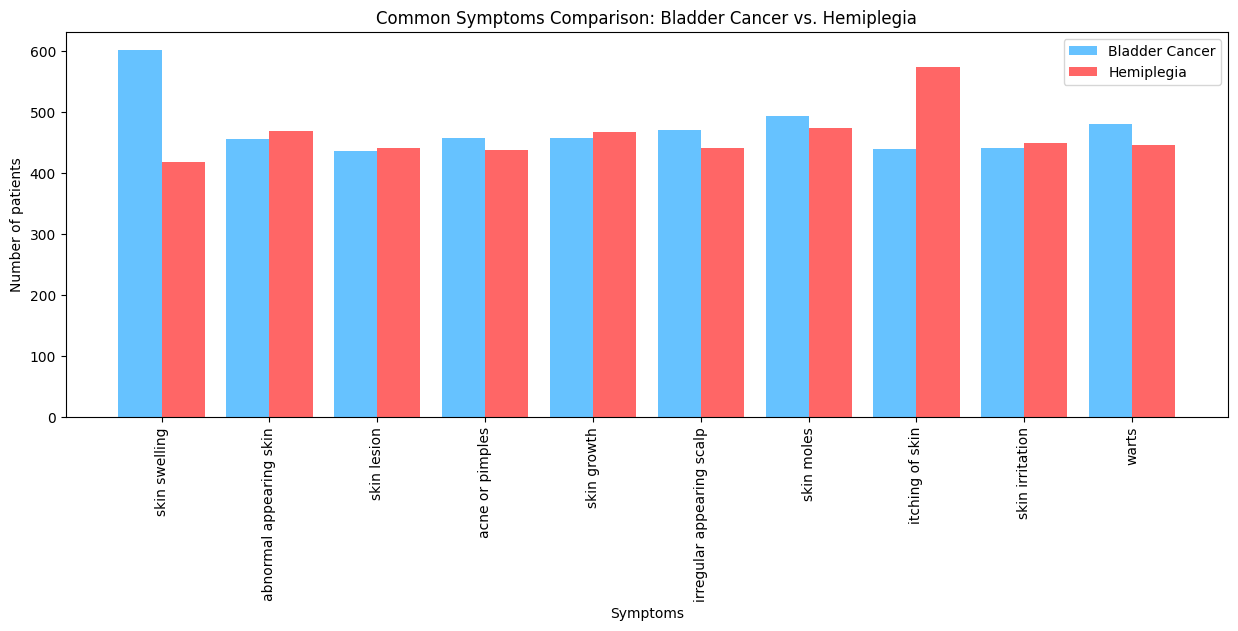
\includegraphics[width=\columnwidth]{cancer_hemiplegia.png}
	\caption{number of samples of bladder cancer and hemiplegia that have the same symptoms}\label{fig:caner_hemiplegia}
\end{figure}
\noindent

\subsubsection*{Analysis of otitis}

In a similar vein, we analyzed otitis, another condition exhibiting low diagnostic accuracy.
Figure\ref{fig:otitis_missclassified} highlights that otitis is frequently misidentified as itching of unknown origin,
with a significant 70\% of cases being incorrectly classified.\\
Figure\ref{fig:otitis_itching} further elucidates this issue,
showing that all otitis samples (100\%) manifest symptoms similar to those of itching of unknown cause.
This overlap in symptoms is a key reason why the model often mistakes otitis for this condition.\\
The challenge in accurately diagnosing otitis is compounded by its minimal representation in the dataset, amounting to only 0.0016\%.
Conversely, itching of unknown cause constitutes a slightly larger portion of the dataset (0.018\%).
This disparity in representation may bias the model towards more frequently diagnosing itching of unknown cause,
leading to the observed high rate (70\%) of misclassification of otitis cases.
\begin{figure}[H]
	\centering
	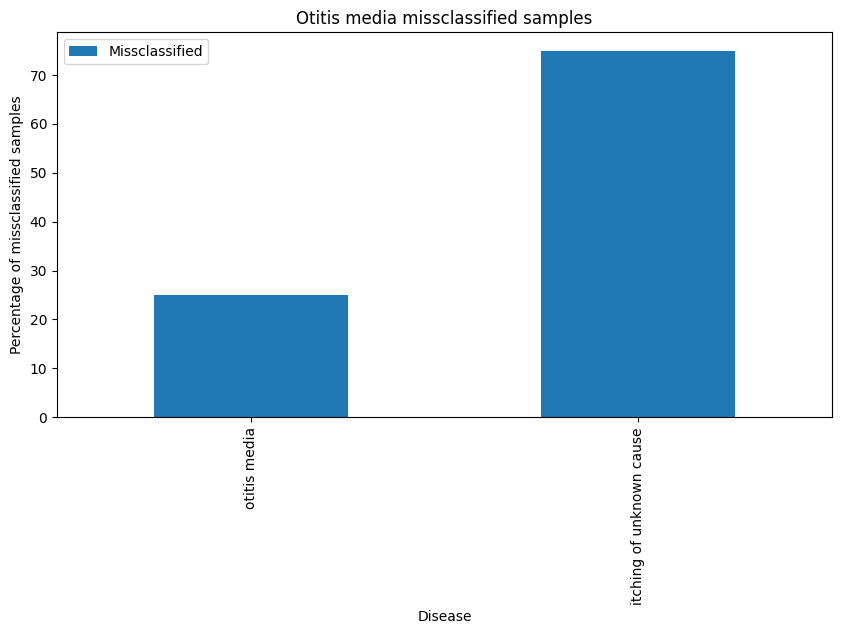
\includegraphics[width=\columnwidth]{otitis_missclassified.png}
	\caption{Percentage of otitis samples misclassified}\label{fig:otitis_missclassified}
\end{figure}
\noindent
\begin{figure}[H]
	\centering
	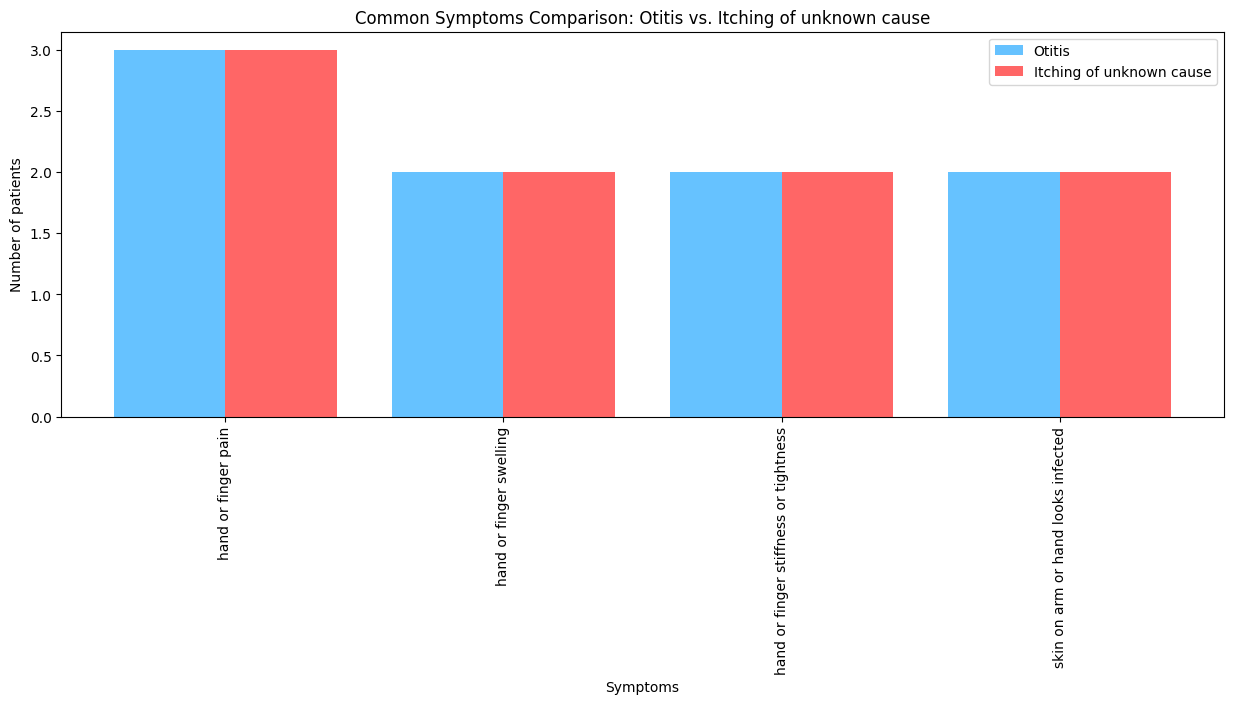
\includegraphics[width=\columnwidth]{otitis_itching.png}
	\caption{number of samples of otitis and itching of unknown cause that have the same symptoms}\label{fig:otitis_itching}
\end{figure}
\noindent

\subsection*{Most impactful symptoms}
Another crucial aspect is to analyze which symptoms are most important for the model.
Since the multiclass version of logistic regression assigns a weight to each symptom for every class,
we have calculated the average absolute value of these weights for each symptom.\\
Figure~\ref{fig:most_important_features} shows the 30 most significant symptoms according to the model.
As can be observed, certain symptoms are more influential. These include both `community size' and `SI index level 2' formats,
such as `sharp chest pain' and `sharp abdominal pain', among others.\\
Furthermore, it is noteworthy that among the three network information types obtained,
none stands out as more important than the others. All three hold significance,
as both `community size' and `SI index level 2' are equally represented among the most important symptoms,
and `community count' is significant for the first two out of three communities.

\begin{figure*}[htbp]
	\centering
	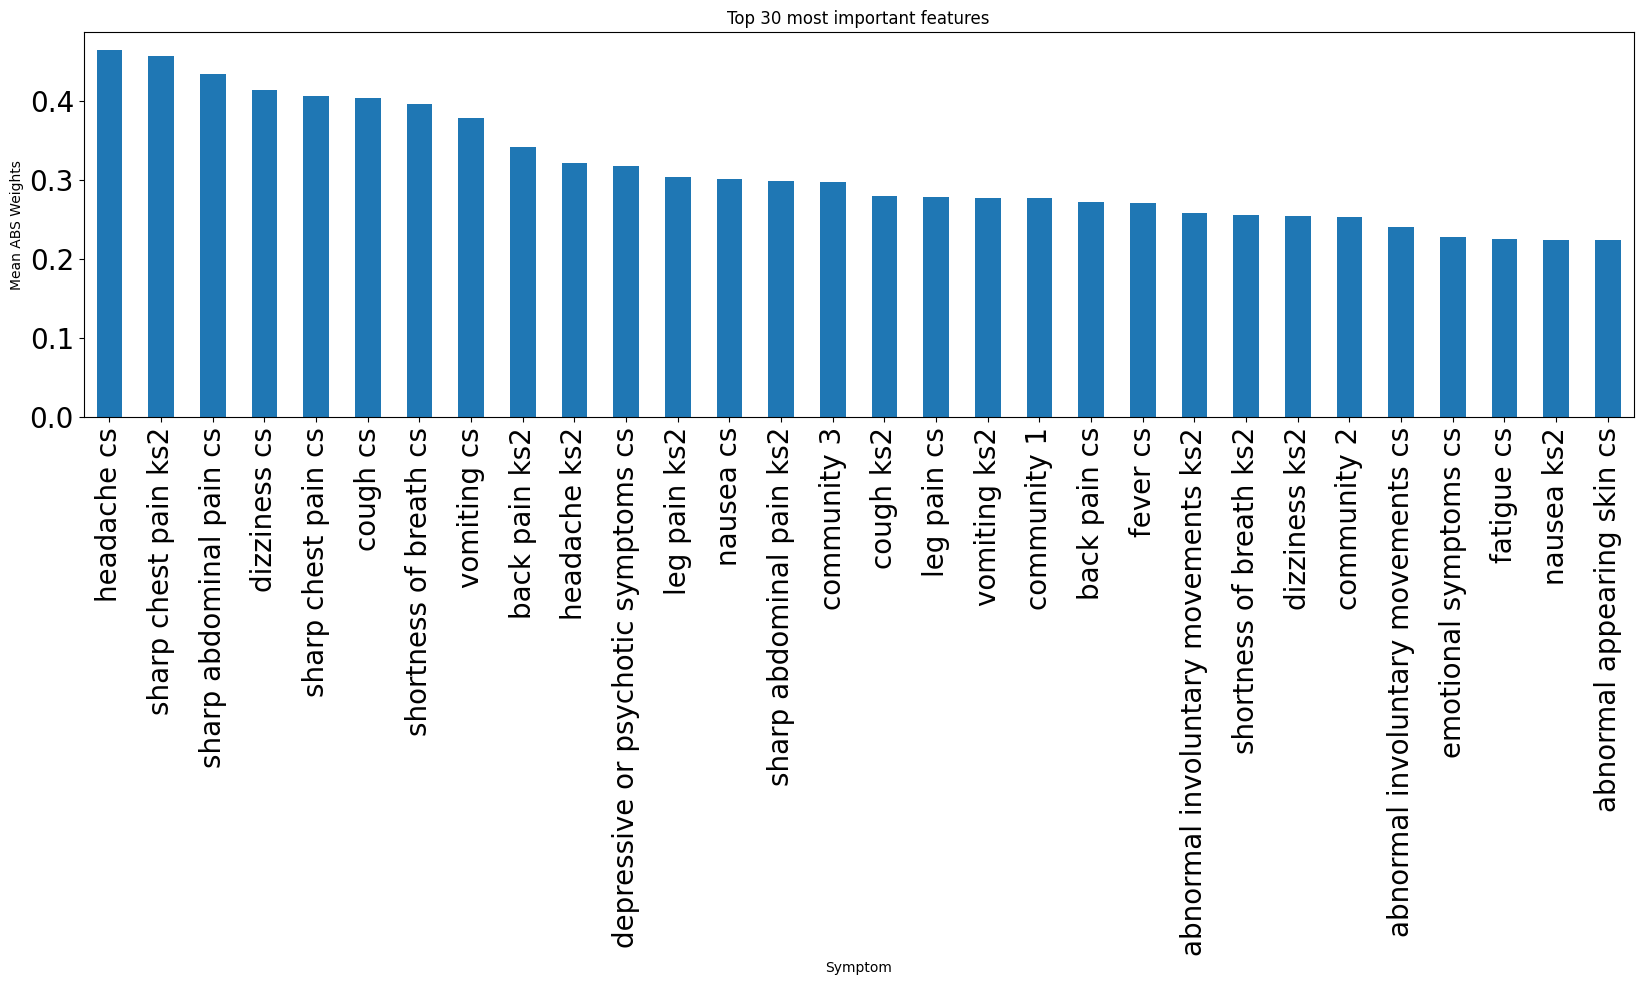
\includegraphics[width=\textwidth]{most_important_features.png}
	\caption{10 most impactful features}\label{fig:most_important_features}
\end{figure*}
\noindent

\subsection{Computational Complexity}
\label{subsec:computational_complexity}
% MATTEO
% - apply the reduction technique based on symptoms importance (L1 and L2 combined in the 4 classes)
% - compare the performance of the reduced model with the original one
% - precision, recall, AUC, accuracy
% - compare the times needed to train the two models
After confirming the presence of some symptoms that are more impactful than others,
we applied a reduction technique based on their importance, leveraging the division
into four classes based on the L1 and L2 Symptom Influence indexes (SI).
The first test was to divide the data into four balanced classes, containing 25\% of the features each.
As shown by Figure~\ref{fig:class_wise_accuracies}, the most impactful set of
features was the one corresponding to the class with both high SI L1 and L2.
This feature class was the one performing better, with only a few classes that were consistently mispredicted.
The worst one was the low-low class, which had a class-wise accuracy of less than 20\% for most of the disease classes.

\begin{figure}[H]
	\centering
	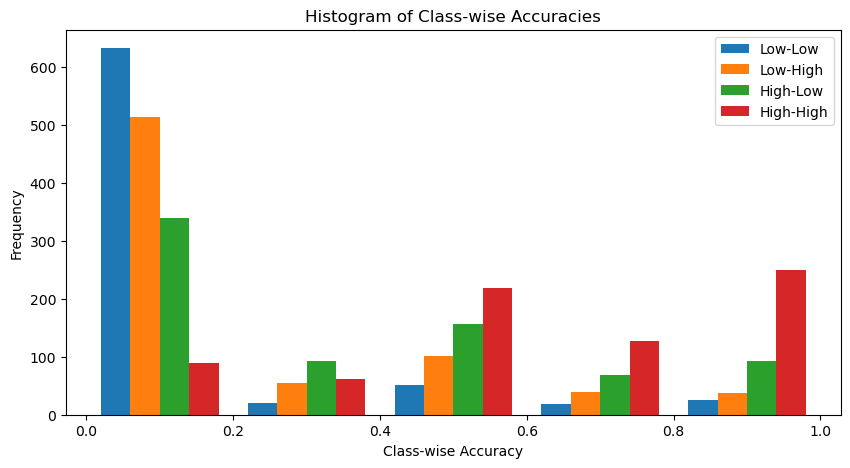
\includegraphics[width=\columnwidth]{class_wise_accuracies.png}
	\caption{Histogram of the class accuracy for each feature group, based on SI L1 and L2.}\label{fig:class_wise_accuracies}
\end{figure}

\noindent
Even then, the high-high class by itself would not be a sufficiently good set of features to make predictions,
so it was used as a baseline to expand the feature set, retaining increasingly more features.
As it can be seen from Figure~\ref{fig:accuracy_vs_features_retained}, the model performance is quite good even when using only
a limited amount of features, reaching around 80\% test accuracy when using half of the features, which corresponds to a
reduction of 10\% of the accuracy of the complete model, giving up half the data.
This is a good trade-off, but the accuracy is valuable, so we decided to give up at most 1\% accuracy,
which in this case corresponds to a reduction of the features by almost 30\%.

\begin{figure}[H]
	\centering
	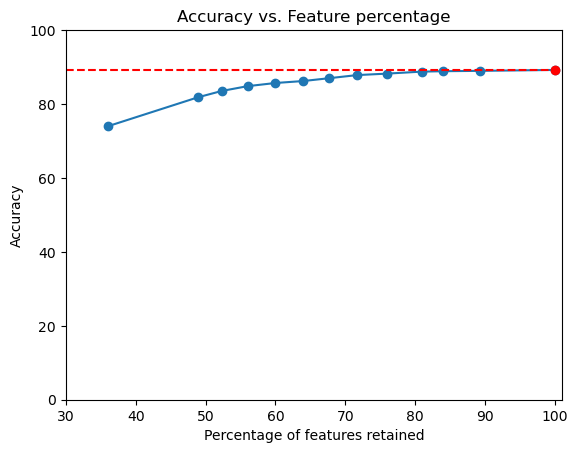
\includegraphics[width=\columnwidth]{accuuracy_vs_features_retained.png}
	\caption{Comparison between the reduction in features against the reduction on the test accuracy.}\label{fig:accuracy_vs_features_retained}
\end{figure}

\noindent
To assess how the reduction of the complexity of the model impacts the training,
we repeated the training phase on the whole balanced dataset, recording the difference in time between the two models.
In the end, the experimental results showed a reduction in training time of 9.39\% caused by a reduction of the training features of 27.87\%.
The relative time reduction is lower in comparison to the whole model, but it shows promising results that
could possibly be even more impactful when dealing with more complex models.

\begin{figure}[H]
	\centering
	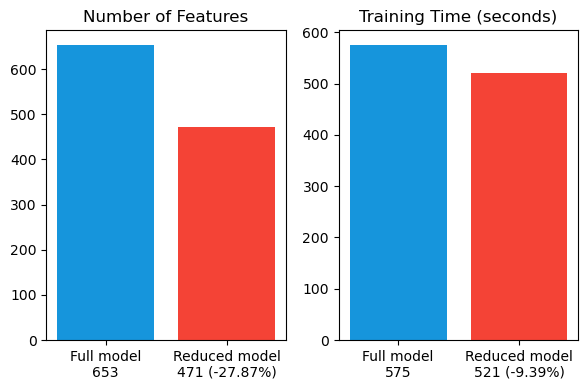
\includegraphics[width=\columnwidth]{features_vs_time.png}
	\caption{Visual rendition of the training time reduction compared to the features.}\label{fig:features_vs_time}
\end{figure}

\noindent
Given the reduction of the features of almost 30\%, the accuracy went down by around a percent and a half,
but to really assess the quality of the reduced model, we cannot rely only on the test accuracy.
Other metrics were employed for the evaluation, which were the precision, recall, and AUC of the ROC.
As depicted by Figure~\ref{fig:precision_recall_auc},
the data showed a similar difference in these metrics, with the exeption of the AUC being almost identical.
This helped us understand that the reduction on the features didn't cause the model to perform well on just the most frequent classes,
but resulted in a good performance across the whole data.

\begin{figure}[H]
	\centering
	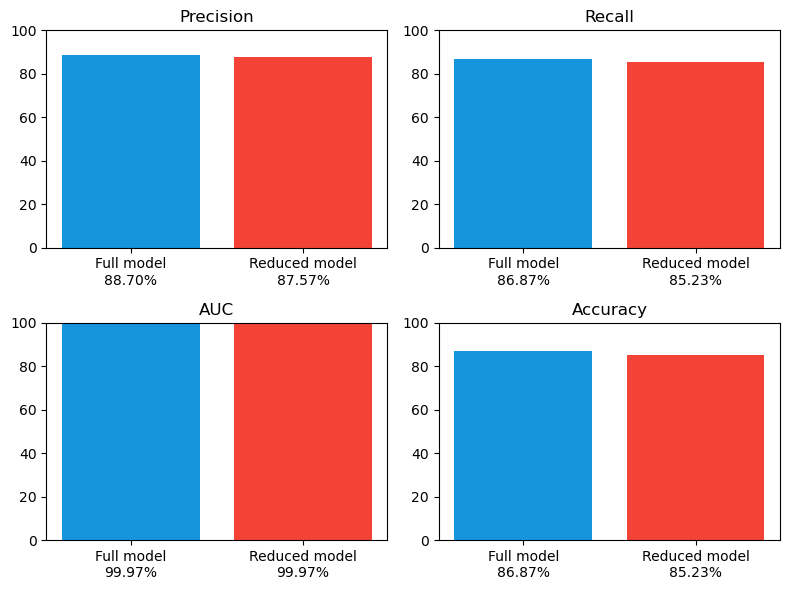
\includegraphics[width=\columnwidth]{precision_recall_auc.png}
	\caption{comparison of various metrics which are useful to asses the relative quality of the reduced model.}\label{fig:precision_recall_auc}
\end{figure}
\noindent

% CRISTIAN
% - 6 Modelli: 3 con solo sintomi, 3 con nuove features
% - - Salvati (joblib) 
% - - Tempo di training


% - selected model performances (see which is the worst error or the most commonly misclassified diseases)
% - Compute accuracy and PR AUC
% - Compute the accuracy of the model dividing the data into the 4 classes (HighL1 - HighL2, LowL1 - HighL2, ...)
% - only with one hot symptoms (with optimal parameters both for one hot and other features) 
% - with new features 
% - reduction in computational complexity

% ---------------------- Conclusion -----------------------------

\section{Conclusion}

Our study successfully integrates network analysis with machine learning to enhance disease prediction models in healthcare.
By analyzing symptom-disease networks using Symptom Influence (SI) and Disease Influence (DI) indices, we uncovered
critical patterns essential for accurate disease prediction. These indices revealed diverse symptom-disease associations,
guiding the selection of features for our models.\\
Logistic Regression emerged as the most effective model, balancing accuracy and complexity, particularly when augmented with network-based features.
This model demonstrated high accuracy and managed to capture complex patterns without significant overfitting.\\
A key achievement of our study is the effective balance between feature reduction and model performance.
Focusing on significant symptoms, we reduced training time substantially while maintaining high accuracy.
This approach is especially valuable in real-world applications where computational efficiency is crucial.\\
The study, however, also recognized challenges in disease prediction, as highlighted by the analysis of specific
diseases like bladder cancer and otitis media. These cases illustrated the intricacies involved in disease classification
and the necessity for continuous model refinement.
\section{Limits and Future Works}
\label{sec:future_works}

In the pursuit of our final model, we navigated through a series of pivotal decisions, ranging from model selection, feature choices, 
and the intricate interplay of normalization techniques to hyperparameter tuning. These decisions, while steering us toward a robust model, 
come with inherent trade-offs, potentially leading to suboptimal outcomes. Here, we discuss some limitations in our approach and suggest 
avenues for future exploration.

\subsection{Limits}
\label{subsec:limits}

\begin{itemize}
\item \textbf{Feature Selection}: The selection of optimal features, as depicted in Figure \ref{fig:ML_operative_flow}, occurred 
before hyperparameter tuning. This sequential approach may result in the choice of an ostensibly optimal feature set, 
as both aspects are tightly linked.

\item \textbf{Hyperparameter Tuning}: The determination of the best hyperparameter combination relied on accuracy as 
the sole metric. While we employed a stratified cross-validation on a balanced dataset for a reliable accuracy estimate, 
a more comprehensive approach should encompass additional metrics such as precision, recall, and F1-score.

\item \textbf{Feature Reduction}: The feature reduction process evenly separated the four classes of symptoms and commenced 
retaining features from the class demonstrating the highest predictive power. This approach may yield suboptimal results, as a 
specific threshold might exist beyond which the predictive power of a feature diminishes. 
To better clarify this concept, let's consider the following example: suppose we have only two classes of symptoms, evenly distributed 
using the median as a threshold on the degree value. Suppose also that the predictive power of the features is the same for both classes.
In this case we cannot actually say that the degree doesn't impact the predictive power of the model. Indeed in the high degree class
we can have put lots of features with a degree not sufficiently high to become less relevant and these diseases end up
altering the result of the whole class, especially in a power law distribution context. 
A refined strategy involves employing a manual threshold for the degree value, identifying truly impactful features, 
potentially resulting in unbalanced classes.

\end{itemize}

\subsection{Future Work}

\begin{itemize}
\item \textbf{Symptoms Communities}: The features extracted from symptom communities were integrated into the model based on their 
inherent ability to capture relevant information. A potential enhancement involves leveraging this knowledge explicitly, using it as prior 
probability for the model. This entails favoring the most common diseases associated with the patient's symptoms and their communities.

\item \textbf{Multi-label Classification}: Our current approach treats diseases as independent entities. However, some diseases 
may be intricately connected. A prospective improvement entails treating diseases as a multi-label classification problem. 
For instance, the model could output the three most likely diseases instead of a singular one.

\item \textbf{Disease Complexity Analysis}: Our accuracy analysis extends to different classes of diseases based on their L1 and L2 values. 
A potential refinement involves a nuanced exploration of disease complexity, adjusting L1 and L2 thresholds to maximize accuracy 
differentials among disease classes. This approach would facilitate an in-depth analysis of diseases that pose higher prediction challenges.

\item \textbf{Rare Diseases}: As shown by the analysis, in many cases the model struggle to predict rare diseases. A valuable future
work could be analyzing the state of the art of rare diseases prediction in literature and try to apply it to our model.

\end{itemize}

% - our approach in feature selection and parameters search is not optimal 
% - list the possible issues (e.g. we are training model on diverse features with the optimal parameters for other features)
% - exploit the knowledge of symptoms communities and their most pointed diseases, using it at prior probability for the model classification

\clearpage
\section{Appendix}

% ------------- Appendix Figures -------------
% Figures to be placed in the appendix

\begin{figure}[H]
	\centering
	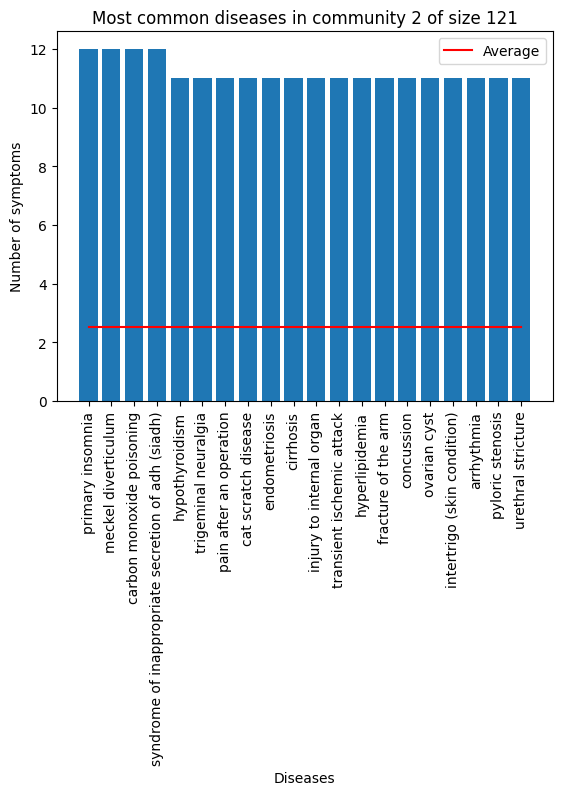
\includegraphics[width=\columnwidth]{com2_symptoms.png}
	\caption{Community 2 of symptoms}\label{fig:com2_symptoms}
\end{figure}
\noindent
\begin{figure}[H]
	\centering
	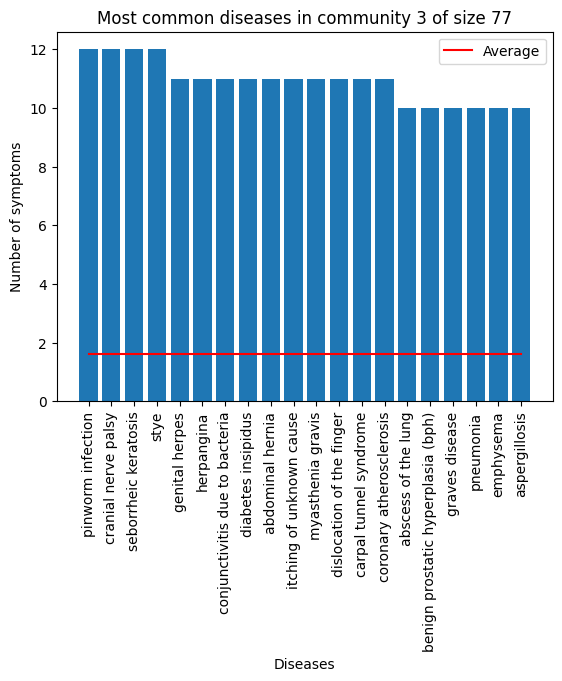
\includegraphics[width=\columnwidth]{com3_symptoms.png}
	\caption{Community 3 of symptoms}\label{fig:com3_symptoms}
\end{figure}
\noindent


\begin{figure}[H]
	\centering
	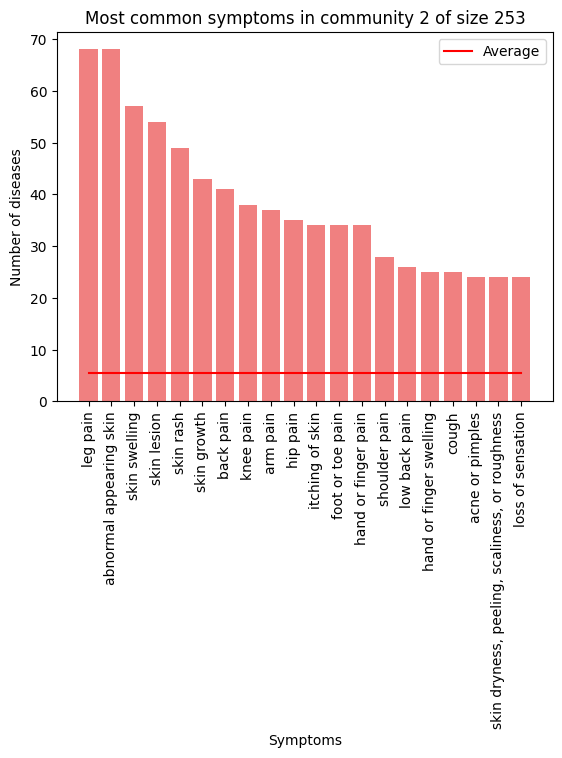
\includegraphics[width=\columnwidth]{com2_diseases.png}
	\caption{Community 2 of diseases}\label{fig:com2_diseases}
\end{figure}
\noindent
\begin{figure}[H]
	\centering
	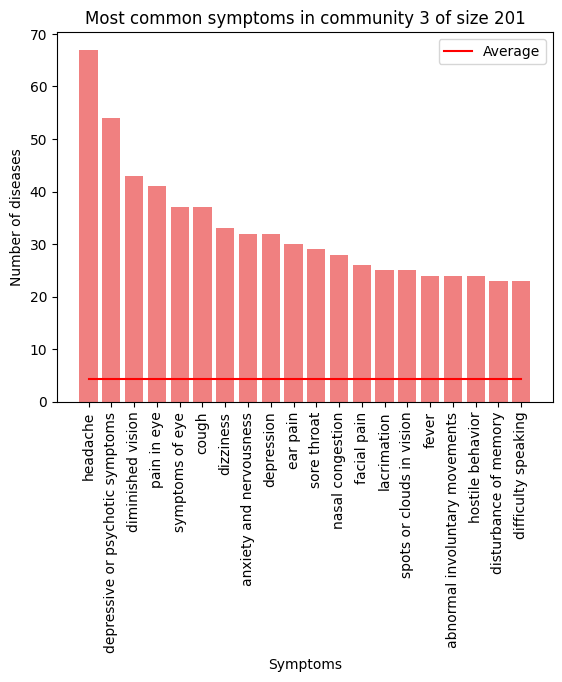
\includegraphics[width=\columnwidth]{com3_diseases.png}
	\caption{Community 3 of diseases}\label{fig:com3_diseases}
\end{figure}
\noindent

\begin{figure*}[!t]
	\centering
	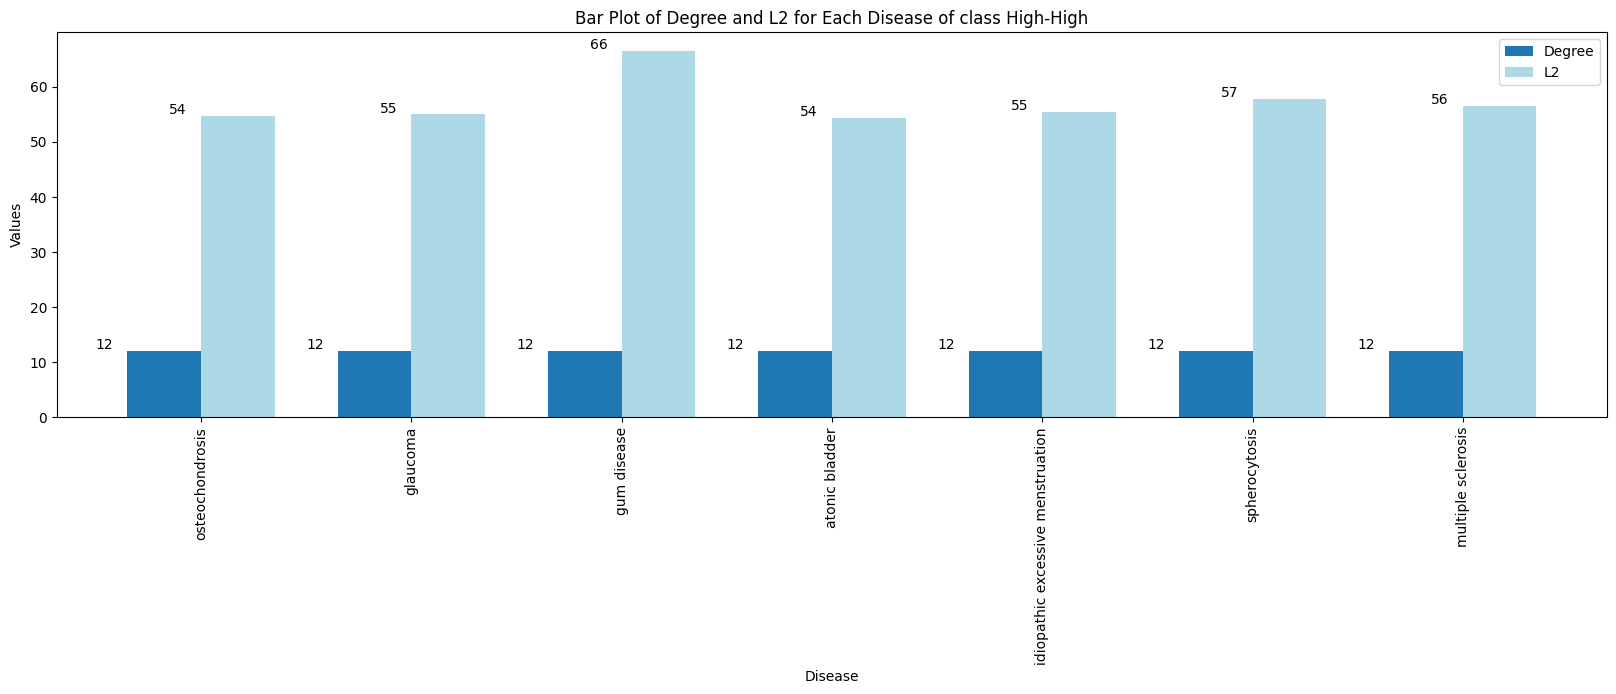
\includegraphics[width=\textwidth]{hig_l1_hig_l2_class.png}
	\caption{Composition of the high-L1-high-L2 class for diseases}\label{fig:high_l1_high_l2_class}
\end{figure*}

\begin{figure}[H]
	\centering
	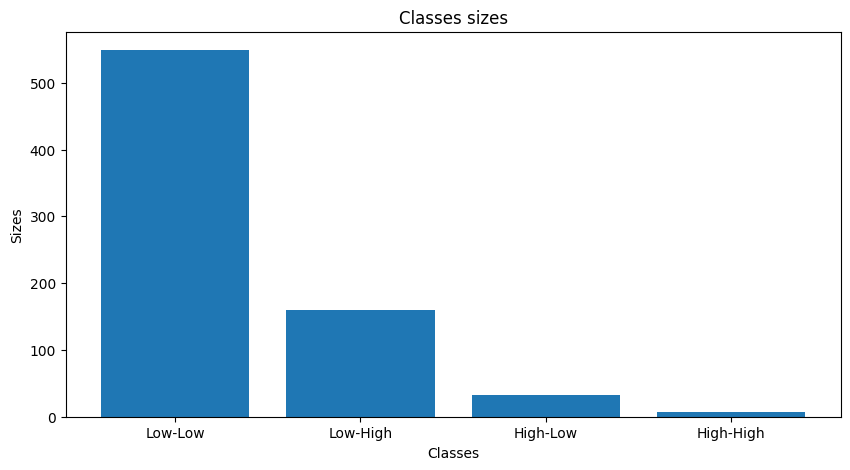
\includegraphics[width=\columnwidth]{diseases_classes.png}
	\caption{Diseases divided into the four classes}\label{fig:diseases_classes}
\end{figure}


\clearpage
\printbibliography

\end{document}